\chapter{(OLD) Beyond SBDRL (to be converted over)}

%%%%%%%%%%%%%%%%%%%%%%%%%%%%%%%%%%%%%%%%%%%%%%%
\section{Action-homogeneous worlds\whendraft{ and generalisation potential}}

\draftnote{blue}{awjdean}{
Hypothesis: action-homogeneous worlds are easier to learn.
Can we design a method that an agent could use to work out the algebra for these worlds ?
Could use the (old) algorithm we developed because each time we move to a new state it's as if we're returning to where we began (kinda - states are still distinct).
}


\whendraft{
	\begin{proposition}
		If $A/\sim$ is a group, then $a' \circ a * w = w$ ($w \in W$, $a, a' \in A/\sim$) does not mean that $a' \circ a * w' = w'$ for all $w' \in W$.
	\end{proposition}
	\begin{proof}
		Proof by counter example.
		Consider the world given in Figure ?
		[insert figure here]
		The algebra of the actions of an agent with minimum actions $\{1, a, b\}$ is given by the following action Cayley table:
		[insert action Cayley table]
	\end{proof}
}

\begin{world_condition}[Action homogeneity]\label{wldcon:action-homogeneity}
	For every pair $(w_{1}, w_{2}) \in W^{2}$, there exists a bijective map $\sigma_{(w_{1},w_{2})}: W \to W$ such that $\sigma_{(w_{1},w_{2})}(w_{1})=w_{2}$ and such that:

	\begin{enumerate}
		\item for every $d \in D_{A}$ with $d: s(d) \xrightarrow{a} t(d)$, there exists a $d' \in D_{A}$ with $d': \sigma_{(w_{1}, w_{2})}(s(d)) \xrightarrow{a} \sigma_{(w_{1}, w_{2})}(t(d))$;

		      % Is this part needed --> implied by first condition due to $\sigma$ being a bijection ?
		\item for every $d \in D_{A}$ with $d: s(d) \xrightarrow{a} t(d)$, there exists a $d' \in D_{A}$ with $d': \sigma^{-1}_{(w_{1}, w_{2})}(s(d)) \xrightarrow{a} \sigma^{-1}_{(w_{1}, w_{2})}(t(d))$.
	\end{enumerate}
\end{world_condition}

World condition ref[wldcon:action-homogeneity] means that action sequences have the same result for any initial world state.
Essentially, this means that the world looks the same from any world state with respect to the relationships of actions.
We call worlds with world condition ref[wldcon:action-homogeneity] \textit{action-homogeneous worlds}.

\begin{definition}[Weak equivalence $\sim_{w}$]\label{def:weak action equivalence}
	For $a,a' \in A$ and $w \in W$, $a \sim_{w} a$ if $a * w = a' * w$ or $a$ and $a'$ are both restricted actions with respect to $w$.
\end{definition}

\begin{remark}
	In definition \ref{def:weak action equivalence}, for the case where $a, a'$ are both restricted actions, then we say $a * w = a' * w$.
	The meaning of $a * w$ where $a$ is restricted on $w$ will be defined later.
\end{remark}

\begin{proposition}
	$\sim_{w}$ is an equivalence relation.
\end{proposition}
\begin{proof}
	To show that $\sim_{w}$ is an equivalence relation, we need to show that the relation is (a) reflexive, (b) transitive, and (c) symmetric.
	(a) For a binary relation $R$ over a set $X$ to be reflexive: $x R x$ for every $x \in X$.
	For $w \in W$, if $a * w$ is defined then $a * w = a * w$ from the properties of $=$ for any $a \in A$.
	Therefore, $a \sim_{w} a$.
	(b) For a binary relation $R$ over a set $X$ to be transitive: if $a R b$ and $b R c$ then $a R c$ for all $a,b,c \in X$.
	If $a \sim_{w} a'$ and $a' \sim_{w} a''$, then $a * w = a' * w$, $a' * w = a'' * w$ for all $w \in W$.
	Combining these two equations gives $a * w = a'' * w$.
	(c) For a binary relation $R$ over a set $X$ to be reflexive: if $a R b$, then $b R a$ for all $a,b \in X$.
	If $a \sim_{w} a'$, then $a * w = a' * w$. Therefore $a' * w = a * w$, and so $a' \sim_{W} a$.
\end{proof}

For action-homogeneous worlds, the following properties hold:
\begin{enumerate}
	\item If a world is action-homogeneous, then $a \sim_{w} a'$ means $a \sim a'$ - this makes it much easier to learn the algebra of action-homogeneous worlds;

	\item The number of elements in $A/\sim$ is always equal to the number of states in the world since for any state $w \in W$, there is exactly one action $a \in A/\sim$ for which $a * w = w'$ where $w'$ is any state in $W$; therefore the number of elements in the action algebra is equal to the number of states in $W$;

	\item If $a * w_{i} = w_{j}$, then there exists a world state $w_{k} \in W$ such that $a * w_{k} = w_{i}$.
	      In other words, if $a$ is defined from one world state it is defined from all world states;

	\item If $a' * (a * w) = a * (a' * w) = w$ for any $w \in W$, then $a' * (a * w) = a * (a' * w) = w$ for all $w \in W$.
	      In other words, reversible actions imply inverse actions.
\end{enumerate}

\whendraft{
	\textbf{[Insert info about generalisation.]}
	\begin{itemize}
		\item If we know that, from a particular initial state, a particular sequence of actions has a particular outcome and we know that a different sequence of actions from the same initial state has the same outcome then we know that those two action sequences will have the same outcome in from every initial state (and therefore will be equivalent?!).
		      \begin{itemize}
			      \item Illustrate this using the counter-example - see PhD Notebook 1 notes.
		      \end{itemize}
	\end{itemize}
}
%%%%%%%%%%%%%%%%%%%%%%%%%%%%%%%%%%%%%%%%%%%%%%%
%%%%%%%%%%%%%%%%%%%%%%%%%%%%%%%%%%%%%%%%%%%%%%%
%%%%%%%%%%%%%%%%%%%%%%%%%%%%%%%%%%%%%%%%%%%%%%%

\section{Beyond SBDRs}\label{sec:Beyond SBDRs}

We will now consider worlds that do not satisfy either world condition ref[wldcon:unrestricted-actions] or world condition ref[wldcon:inverse-actions] and so have transformations that do not form a group action.
We have selected examples with features that are common in simple reinforcement learning scenarios.

We also consider two methods of treating actions that are not allowed to be used in certain world states (\textit{e.g.}, the agent trying to move through a wall or eat a consumable in a state where the agent is not in the same location as a consumable).
Method 1 (Sections ref[sec:identity reversible action-inhomogeneous world] and ref[sec:identity irreversible inhomogeneous actions]) lets the agent select the actions but any actions that would have been undefined in a state $w$ have the same effect in $w$ as the agent performing the identity action $1$.
Method 2 (Sections ref[sec:masked reversible action-inhomogeneous world] and ref[sec:masked irreversible action-inhomogeneous world]) does not let the agent select these actions and so considers them as undefined; this violates world condition ref[wldcon:unrestricted-actions].
These two treatments of actions are commonly used in reinforcement learning.
We use the computational methods outlined in Section ref[sec:Algorithmic exploration of world structures] to generate the action algebras of the agent in these worlds and provide evidence for our statements.

We also prove that the treatment of actions affects the algebra of the world (Proposition ref[prp:algebra$\_$depends$\_$on$\_$action$\_$treatment]).

%%%%%%%%%%%%%%%%%%%%%%%%%%%%%%%%%%%%%
\subsection{Beyond groups}

If we relax one or more of the properties of a group, then we get more general algebraic structures.
The relevant algebraic structures and their properties are shown in Table \ref{tab:group-like-algebraic-structures}.

\begin{table}[H]
    \centering
    \begin{tabular}{c|c|c|c|c}
                        & Closure   & Identity & Inverse  & Associativity \\
                        \hline
                        &           &          &          & \\
        Group           & Y         & Y        & Y        & Y \\
                        &           &          &          & \\
        Monoid          & Y         & Y        & N        & Y \\
                        &           &          &          & \\
        Small category  & N         & Y        & N        & Y \\
                        &           &          &          & \\
    \end{tabular}
    \caption{The group properties of relevant group-like algebraic structures.}
    \label{tab:group-like-algebraic-structures}
\end{table}

%%%%%%%%%%%%%%%%%%%%%%%%%%%%%%%%%%%%%%%%%%%%%%%%%%%%%%%%%%%%%%%%%%%%%%%%%%%%%
\subsection{Worlds without inverse actions}

In this section, we consider worlds that do not necessarily satisfy world condition ref[wldcon:inverse-actions] but do satisfy world condition ref[wldcon:unrestricted-actions].

\begin{proposition}\label{prp:wc1_gives_monoid_action}
    Consider a world $\mathscr{W}$ with a set $W$ of world states and containing an agent with a set $A$ of actions.
    If $\mathscr{W}$ satisfies world condition ref[wldcon:unrestricted-actions], then $*: (A/\sim) \times W \to W'$, where $W' \subseteq W$, is the action of a monoid $A/\sim$ on $W$.
\end{proposition}
\begin{proof}
    (1) Totality of $A/\sim$ is given by world condition ref[wldcon:unrestricted-actions].
    (2) Associativity of $A/\sim$ is given by proposition ref[prp:Asim-associative].
    (3) Identity element of $A/\sim$ is given by proposition ref[prp:Asim-identity].
    Since $A/\sim$ satisfies properties (1), (2), and (3), $A/\sim$ is a monoid.
    
    $*$ is defined for any $a \in A$ and $w \in W$, therefore $*$ is a monoid action.
\end{proof}

\begin{remark}
    If all actions are reversible in $\mathscr{W}$ then $W' = W$.
    If any action is irreversible in $\mathscr{W}$ then $W' \subset W$.
\end{remark}

%%%%%%%%%%%%%%%%%%%%%%%%%%%%%%%%%%%%%%%%%%%%%%%%%%%%%%%%%%%%%%%%%%%%%%%%%%%
\subsection{Example 1: reversible action-inhomogeneous world}\label{sec:identity reversible action-inhomogeneous world}

To turn the $2 \times 2$ cyclical grid world $\mathscr{W}_{c}$ used previously from a reversible action-homogeneous world to a reversible action-inhomogeneous world we add a wall to the world as shown in Figure \ref{fig:2x2-cyclical-grid-world-wall-states} to give world $\mathscr{W}_{wall}$.

\begin{figure}[H]
  \centering
    \begin{subfigure}[b]{0.45\linewidth}
        \centering
        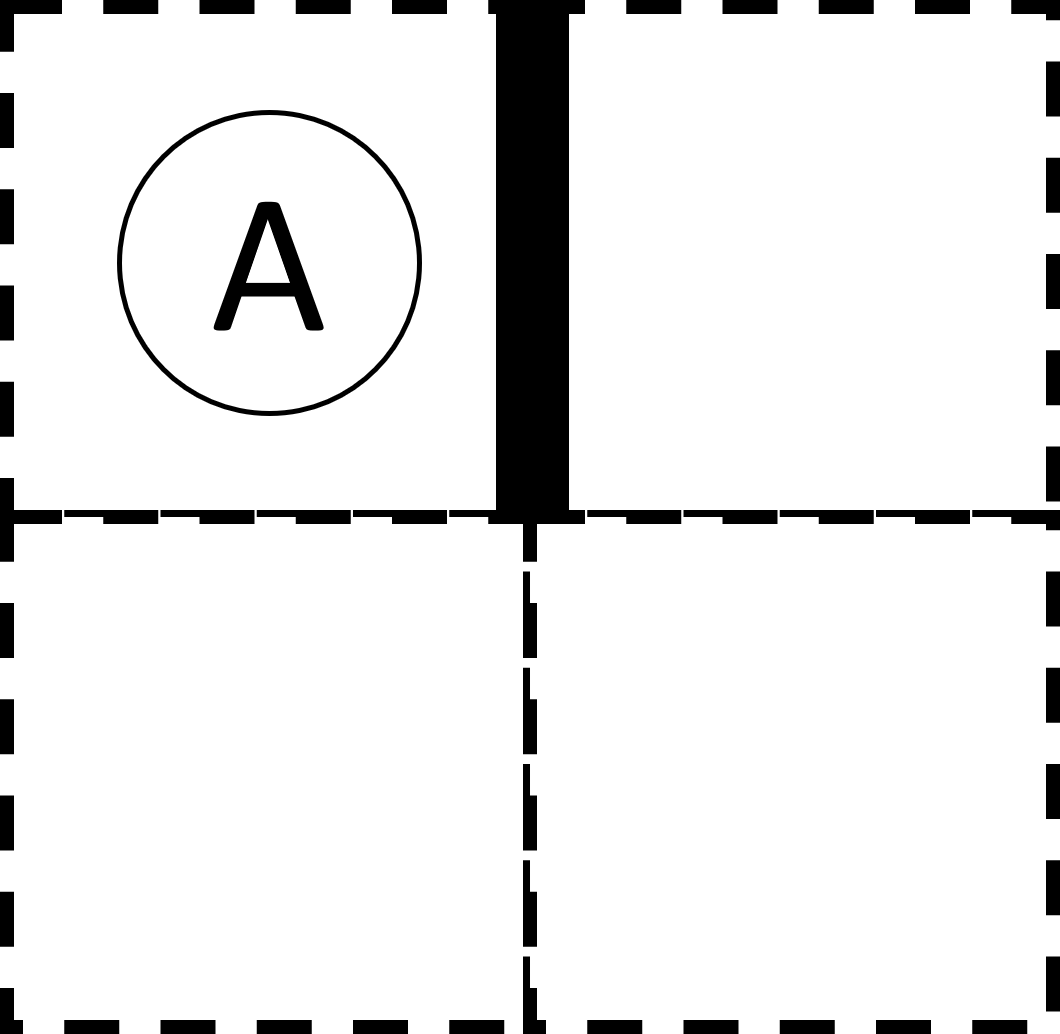
\includegraphics[width=0.5\linewidth]{5BeyondSBDRL/Old/Images/2x2_with_wall_world_states/w0.png}
        \caption{$w_{0}$}
        \vspace{0.25cm}
    \end{subfigure}
    \begin{subfigure}[b]{0.45\linewidth}
        \centering
        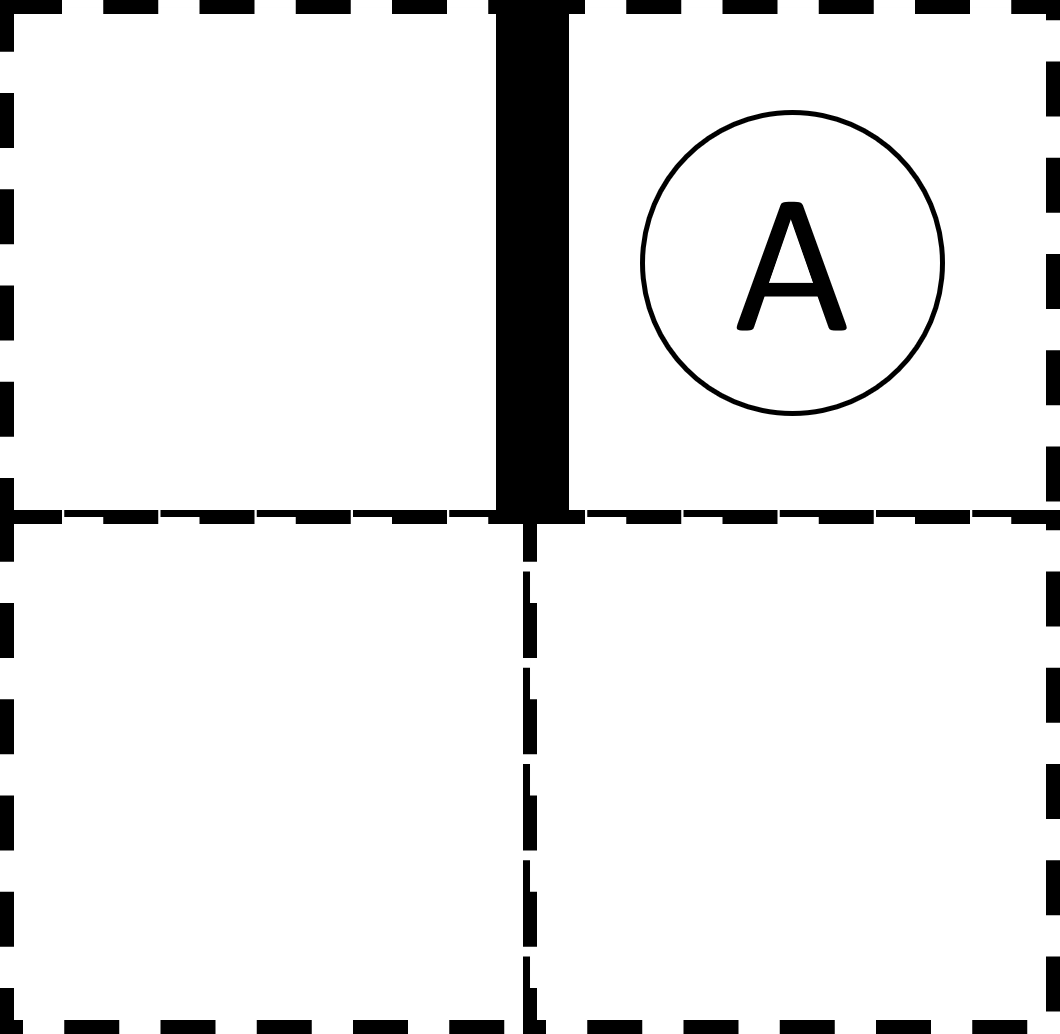
\includegraphics[width=0.5\linewidth]{5BeyondSBDRL/Old/Images/2x2_with_wall_world_states/w1.png}
        \caption{$w_{1}$}
        \vspace{0.25cm}
    \end{subfigure}
    \begin{subfigure}[b]{0.45\linewidth}
        \centering
        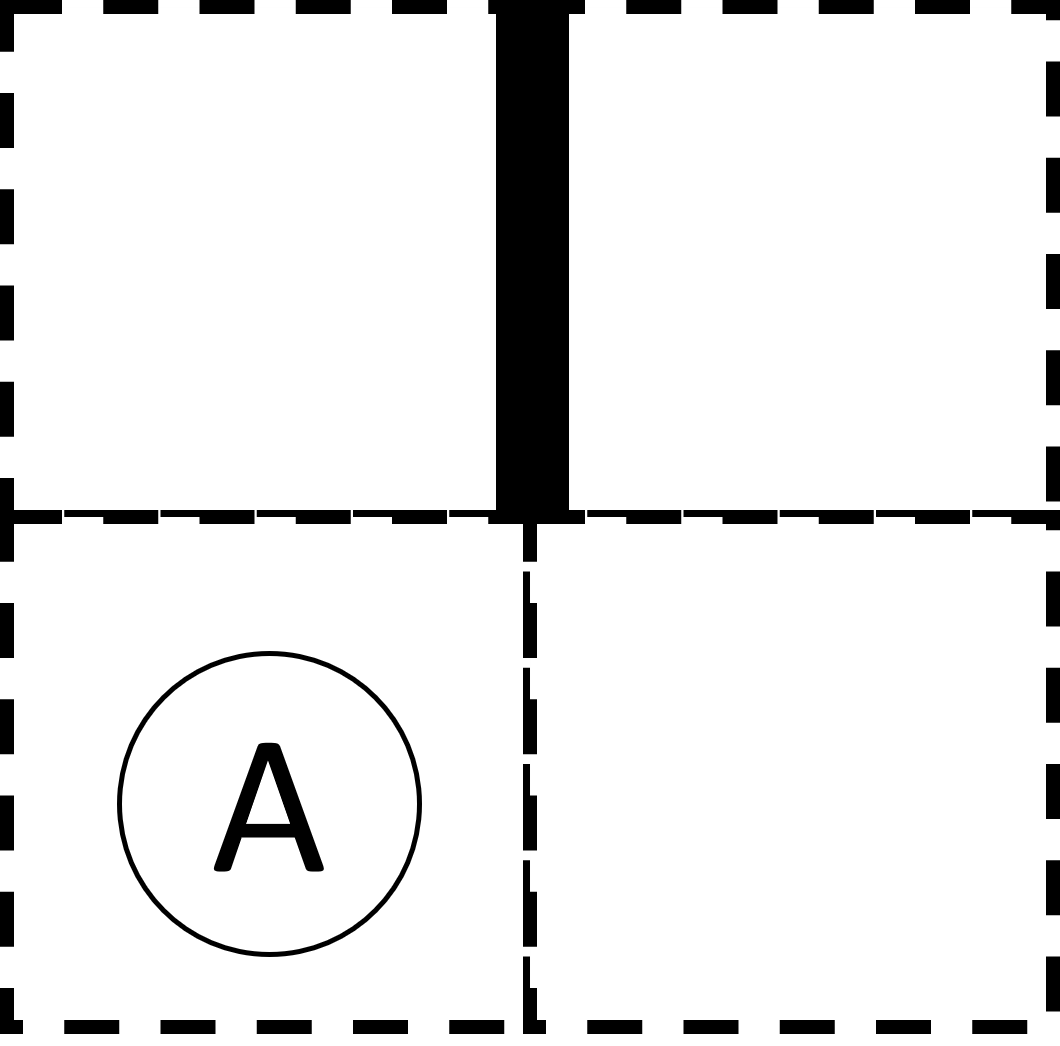
\includegraphics[width=0.5\linewidth]{5BeyondSBDRL/Old/Images/2x2_with_wall_world_states/w2.png}
        \caption{$w_{2}$}
    \end{subfigure}
    \begin{subfigure}[b]{0.45\linewidth}
        \centering
        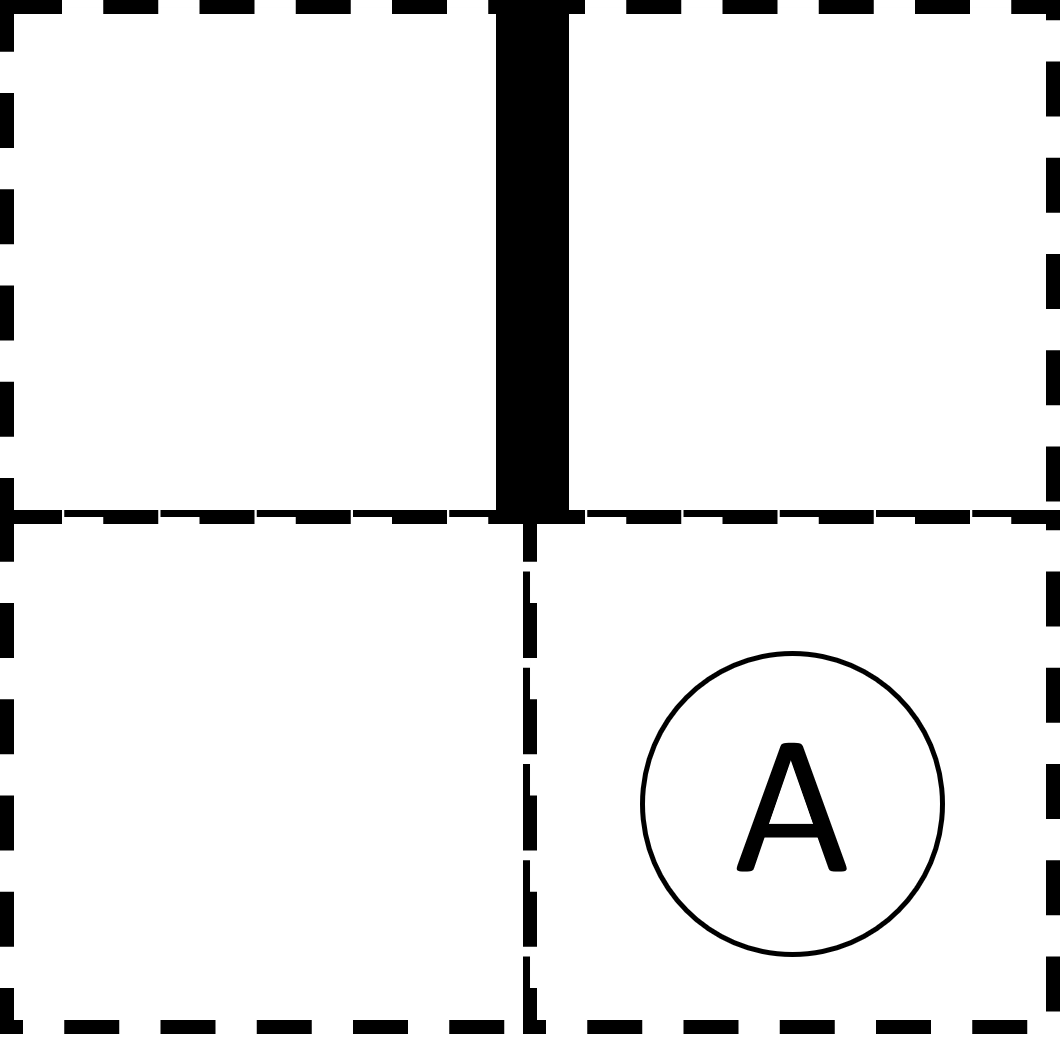
\includegraphics[width=0.5\linewidth]{5BeyondSBDRL/Old/Images/2x2_with_wall_world_states/w3.png}
        \caption{$w_{3}$}
    \end{subfigure}
  \caption{
  The world states of a cyclical $2\times 2$ grid world $\mathscr{W}_{wall}$ with a wall, where changes to the world are due to an agent moving either up, down, left, or right.
  The position of the agent in the world is represented by the position of the circled A.
  The treatment of the wall is explained when needed.
  }
  \label{fig:2x2-cyclical-grid-world-wall-states}
\end{figure}

This wall is said to \textit{restrict} the actions of the agent.
We say that actions restricted by the wall affect the world in the same way as the identity action; for example, if the agent is directly to the left of a wall and performs the `move to the right' action, then this action is treated like the identity action and so the state of the world does not change (see Table \ref{tab:2x2-gridworld-minimum-transitions-wall-identity} and Figure \ref{fig:2x2-cyclical-min-actions-wall-identity}).

\begin{table}[H]
    \centering
    \begin{tabular}{c|c c c c c}
                &  $1$      & $U$       & $D$       & $L$               & $R$\\
         \hline
        $w_{0}$ & $w_{0}$   & $w_{2}$   & $w_{2}$   & $w_{1}$           & \textbf{$w_{0}$}\\
        $w_{1}$ & $w_{1}$   & $w_{3}$   & $w_{3}$   & \textbf{$w_{1}$}  & $w_{0}$\\
        $w_{2}$ & $w_{2}$   & $w_{0}$   & $w_{0}$   & $w_{3}$           & $w_{3}$\\
        $w_{3}$ & $w_{3}$   & $w_{1}$   & $w_{1}$   & $w_{2}$           & $w_{2}$\\
    \end{tabular}
    \caption{
    Each entry in this table shows the outcome state of the agent performing the action given in the column label when in the world state given by the row label.
    }
    \label{tab:2x2-gridworld-minimum-transitions-wall-identity}
\end{table}

\begin{figure}
    \centering
    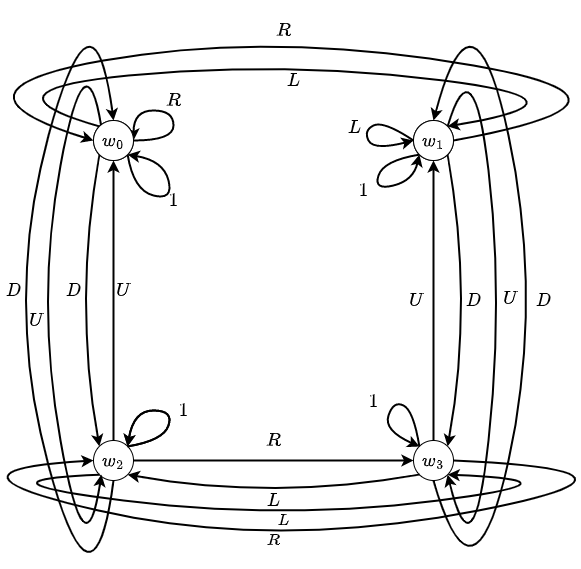
\includegraphics[width=0.5\linewidth]{5BeyondSBDRL/Old/Images/identity-walls-2x2-cyclical-min-actions.drawio.png}
    \caption{
    A transition diagram of the labelled transitions in Table \ref{tab:2x2-gridworld-minimum-transitions-wall-identity}.
    }
    \label{fig:2x2-cyclical-min-actions-wall-identity}
\end{figure}

\paragraph{Properties and structure of $A/\sim$}
The action Cayley table for this world with the identity treatment of the walls contains 26 elements.
As shown in Table \ref{tab:identity-walls-properties}, $A/\sim$ is a monoid.

\begin{table}[H]
    \centering
    \begin{tabular}{c|c}
        \textbf{Property}   & \textbf{Present?} \\
        \hline
        Totality            & Y\\
        Identity            & Y\\
        Inverse             & N\\
        Associative         & Y\\
        Commutative         & Y
    \end{tabular}
    \caption{Properties of the $A/\sim$ algebra.}
    \label{tab:identity-walls-properties}
\end{table}

Adding a single wall to the world has massively increased the complexity of the transition algebra of the world.
While the transition algebra of $\mathscr{W}_{c}$ has four elements, the transition algebra of $\mathscr{W}_{wall}$ with restricted actions treated as identity actions contains 26 elements.

The restrictiveness of the group inverse condition should be noted.
For $\mathscr{W}_{wall}$ with restricted actions treated as identity actions, every action is reversible from a particular state $w \in W$.
However, the action that takes $a$ back to its starting state is not necessarily the same any starting state $w \in W$.
For the inverse property to be present, the inverse for each element must be the same from any starting state (\textit{i.e.}, the inverse must be independent of the starting state).
$\mathscr{W}_{wall}$ with restricted actions treated as identity actions is proof that it is possible to have a world where all actions are reversible but for some of those actions to not have an inverse action.


%%%%%%%%%%%%%%%%%%%%%%%%%%%%%%%%%%%%%%%%%%
\subsection{Example 2: Reversible action-inhomogenous world without walls}

Consider a world $\mathscr{W}_{block}$ with the world states in Figure \ref{fig:movable_block_world_states} and with movement along a single 1D cyclical axis with a movable block.
If the agent is in the location directly to the left of the block and moves into the block, the block moves one location in the direction of the agent's movement and the agent moves into the location previously occupied by the block (see Table \ref{tab:4x1-gridworld-minimum-transitions-moveable-block} and Figure \ref{fig:4x1-block-min-actions-wall}).

\begin{figure}[htbp]
  \centering
  \begin{subfigure}{0.48\textwidth}
    \centering
    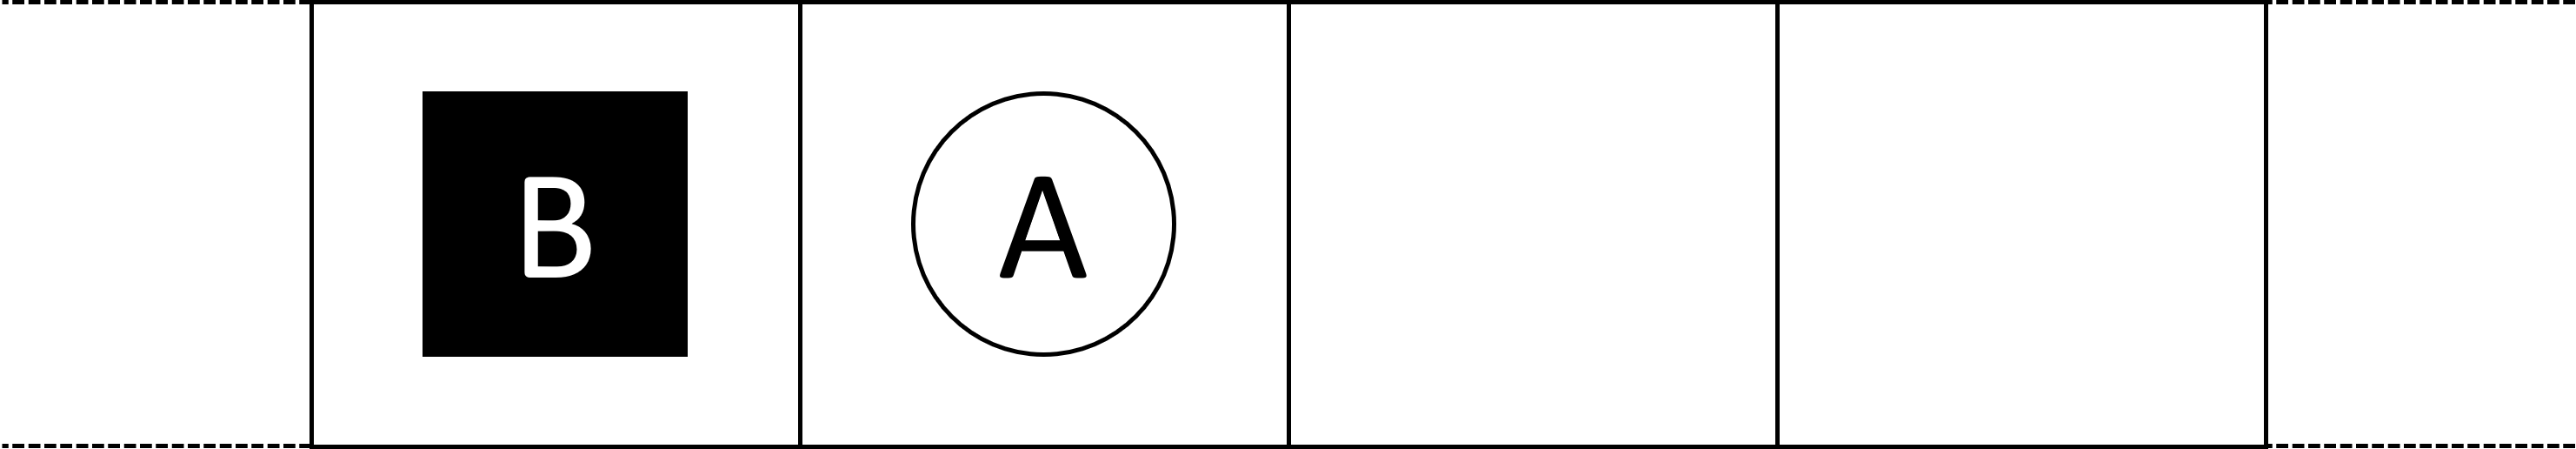
\includegraphics[width=\textwidth]{5BeyondSBDRL/Old/Images/Movable_block_world_states/w0.png}
    \caption{$w_{0}$}
  \end{subfigure}%
  \hfill
  \begin{subfigure}{0.48\textwidth}
    \centering
    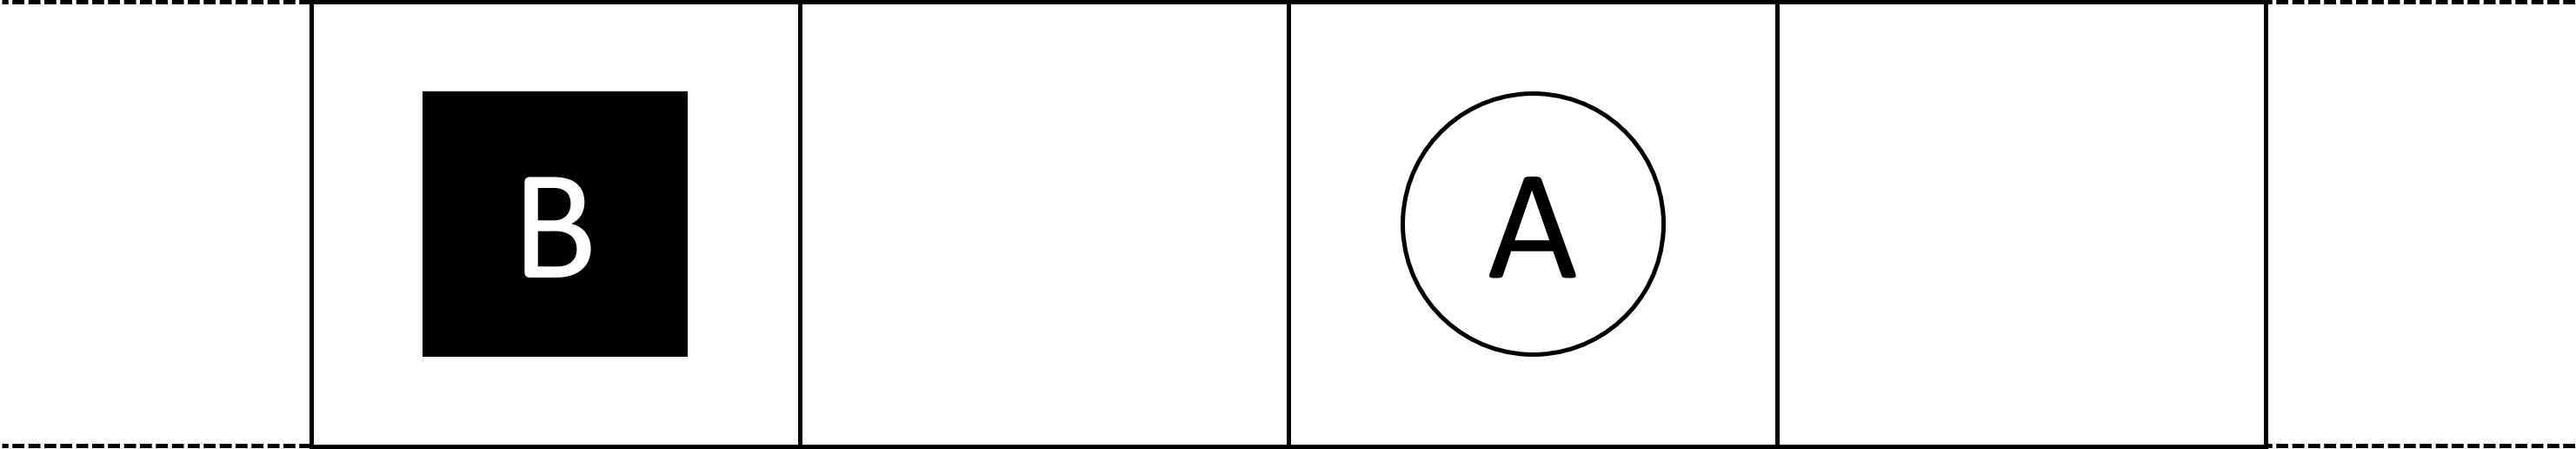
\includegraphics[width=\textwidth]{5BeyondSBDRL/Old/Images/Movable_block_world_states/w1.png}
    \caption{$w_{1}$}
  \end{subfigure}%
  \vspace{0.5cm}
  \begin{subfigure}{0.48\textwidth}
    \centering
    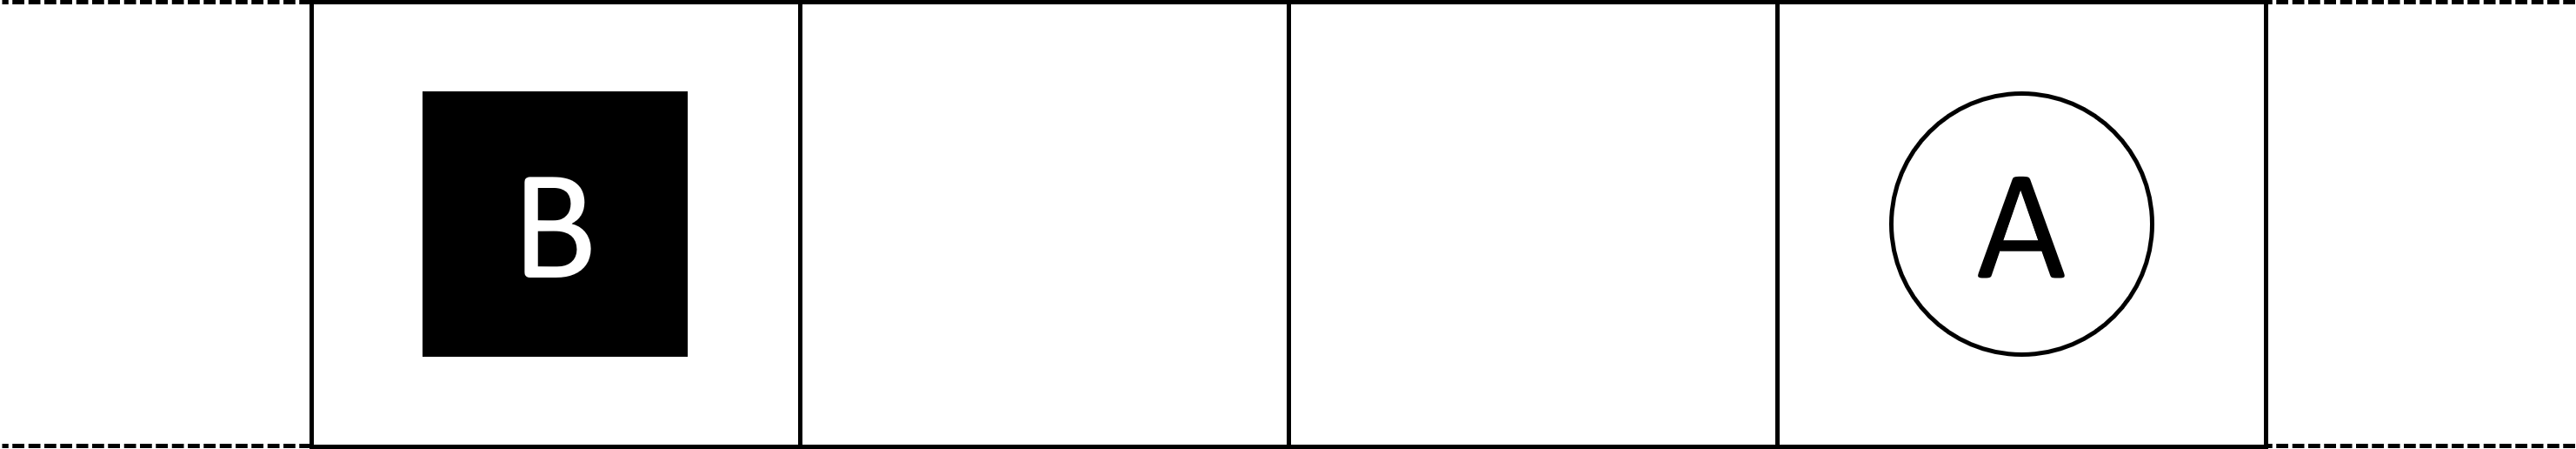
\includegraphics[width=\textwidth]{5BeyondSBDRL/Old/Images/Movable_block_world_states/w2.png}
    \caption{$w_{2}$}
  \end{subfigure}%
  \hfill
  \begin{subfigure}{0.48\textwidth}
    \centering
    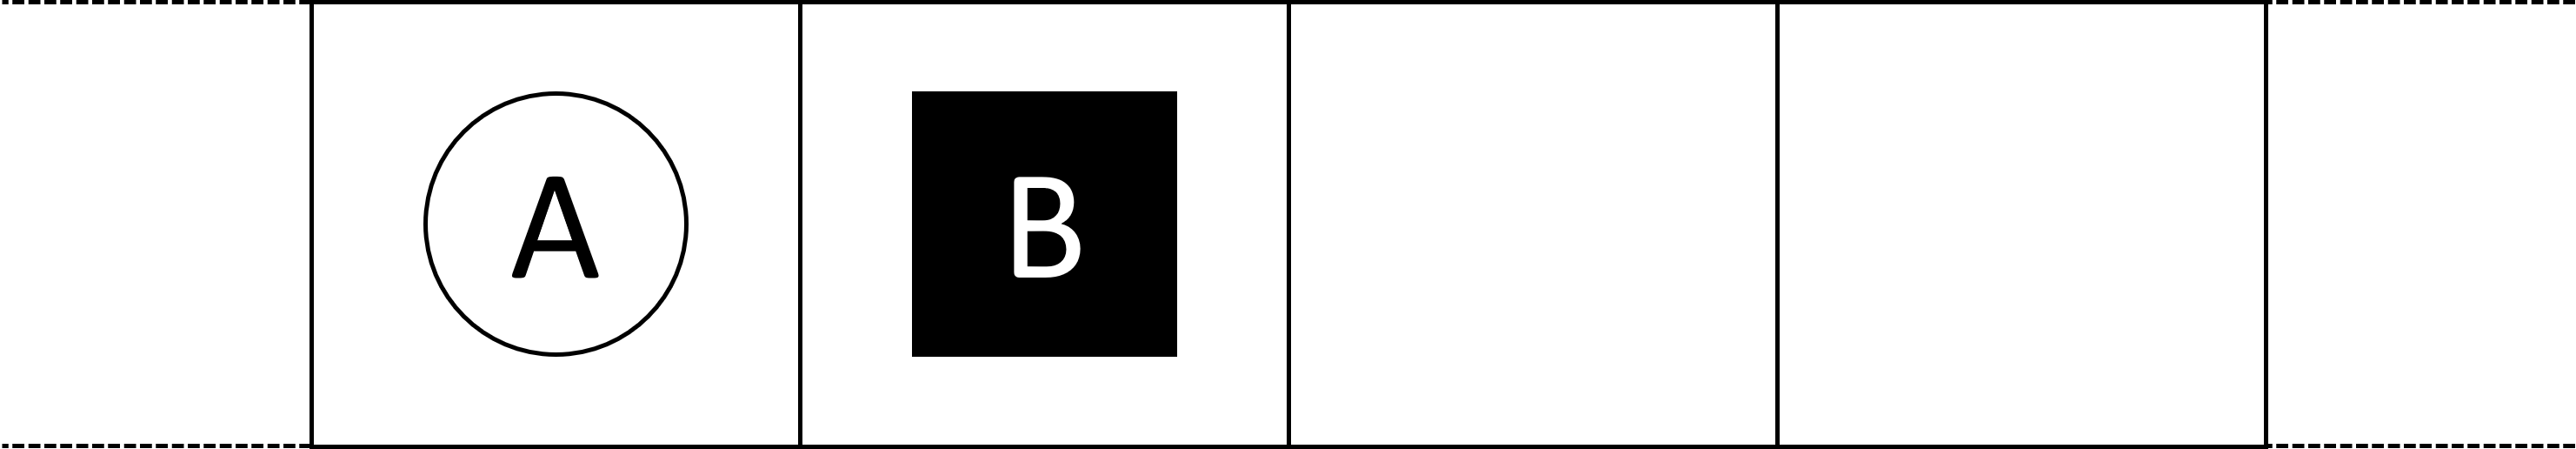
\includegraphics[width=\textwidth]{5BeyondSBDRL/Old/Images/Movable_block_world_states/w3.png}
    \caption{$w_{3}$}
  \end{subfigure}%
  \vspace{0.5cm}
  \begin{subfigure}{0.48\textwidth}
    \centering
    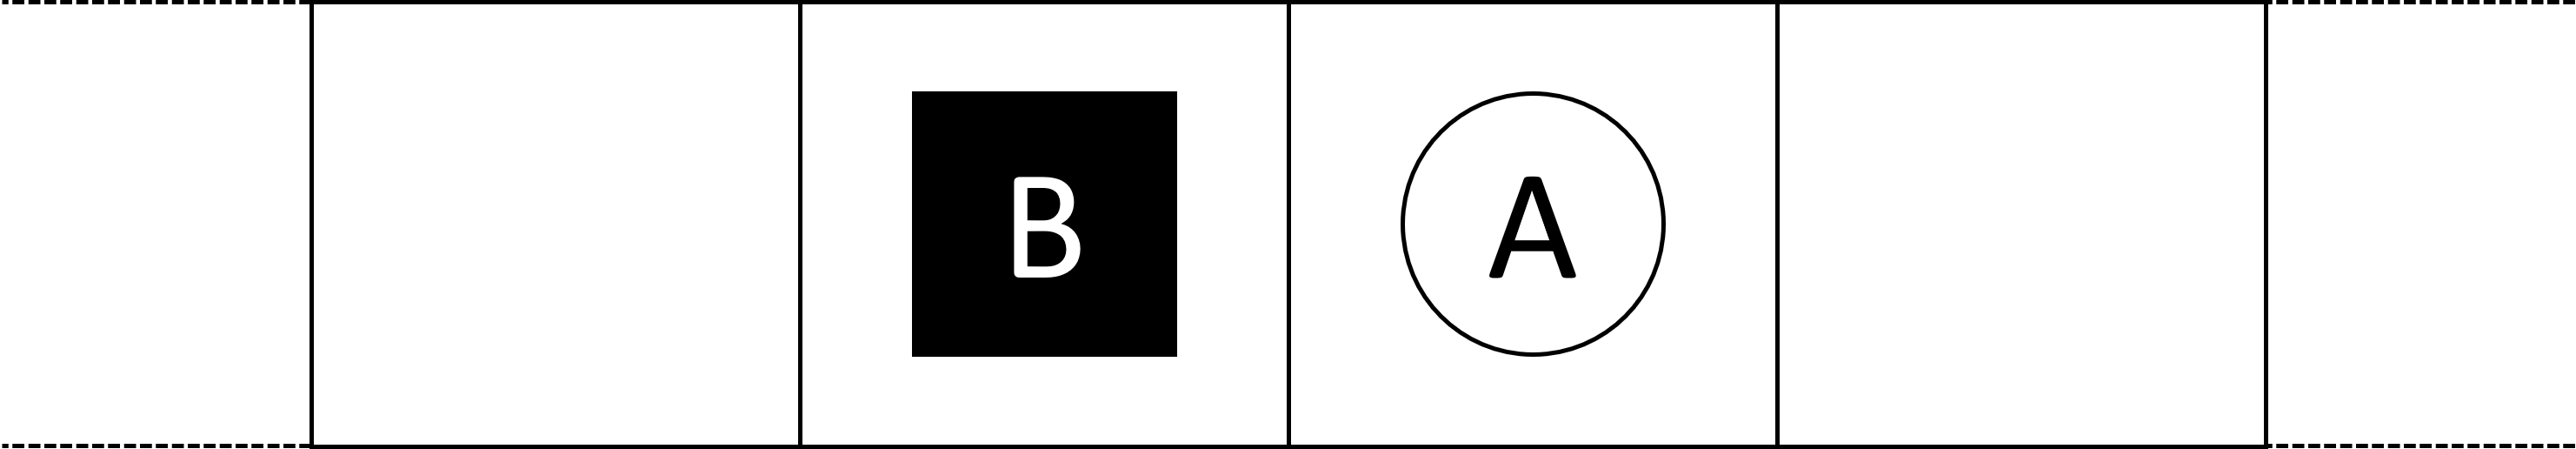
\includegraphics[width=\textwidth]{5BeyondSBDRL/Old/Images/Movable_block_world_states/w4.png}
    \caption{$w_{4}$}
  \end{subfigure}%
  \hfill
  \begin{subfigure}{0.48\textwidth}
    \centering
    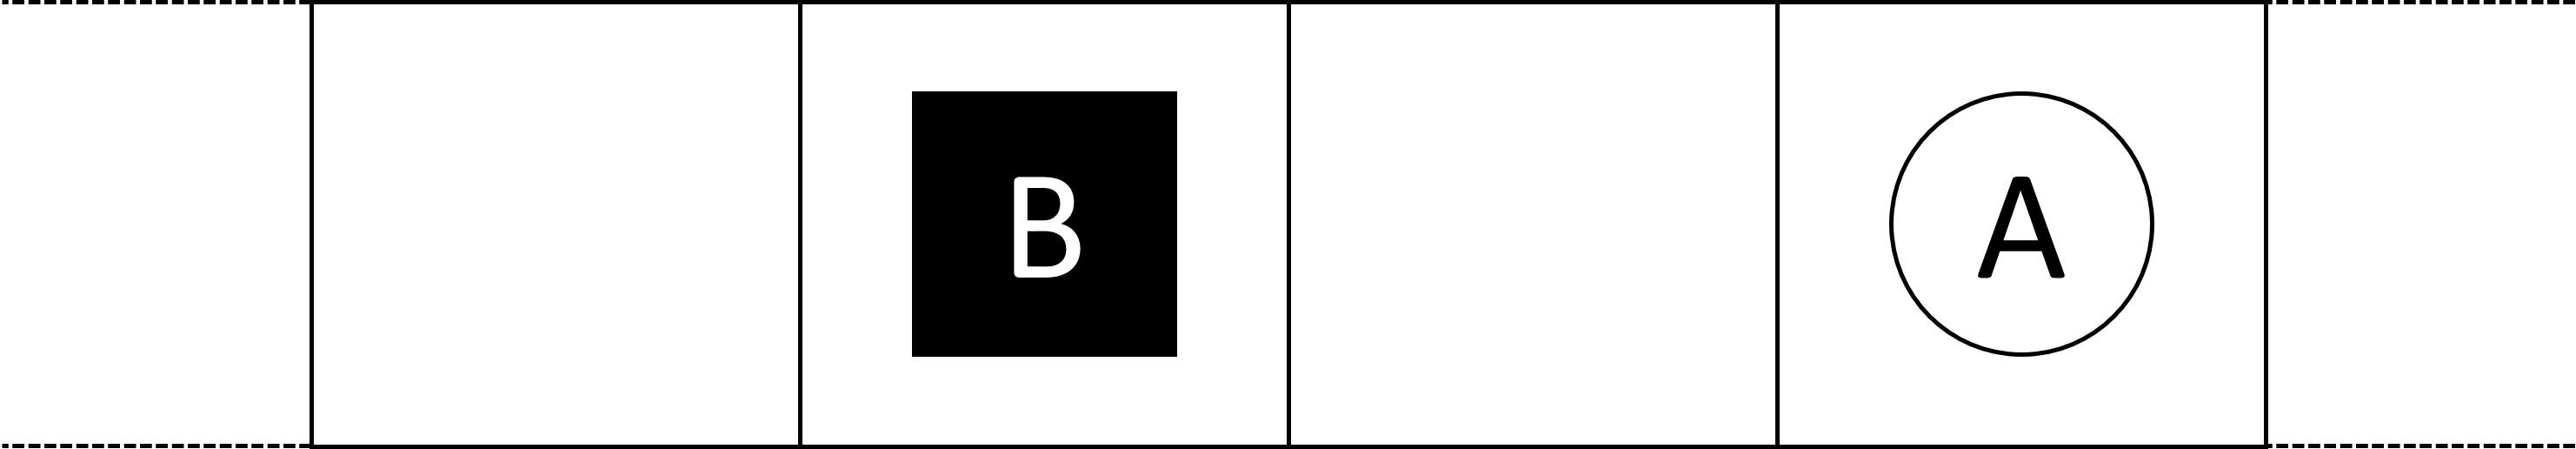
\includegraphics[width=\textwidth]{5BeyondSBDRL/Old/Images/Movable_block_world_states/w5.png}
    \caption{$w_{5}$}
  \end{subfigure}%
  \vspace{0.5cm}
  \begin{subfigure}{0.48\textwidth}
    \centering
    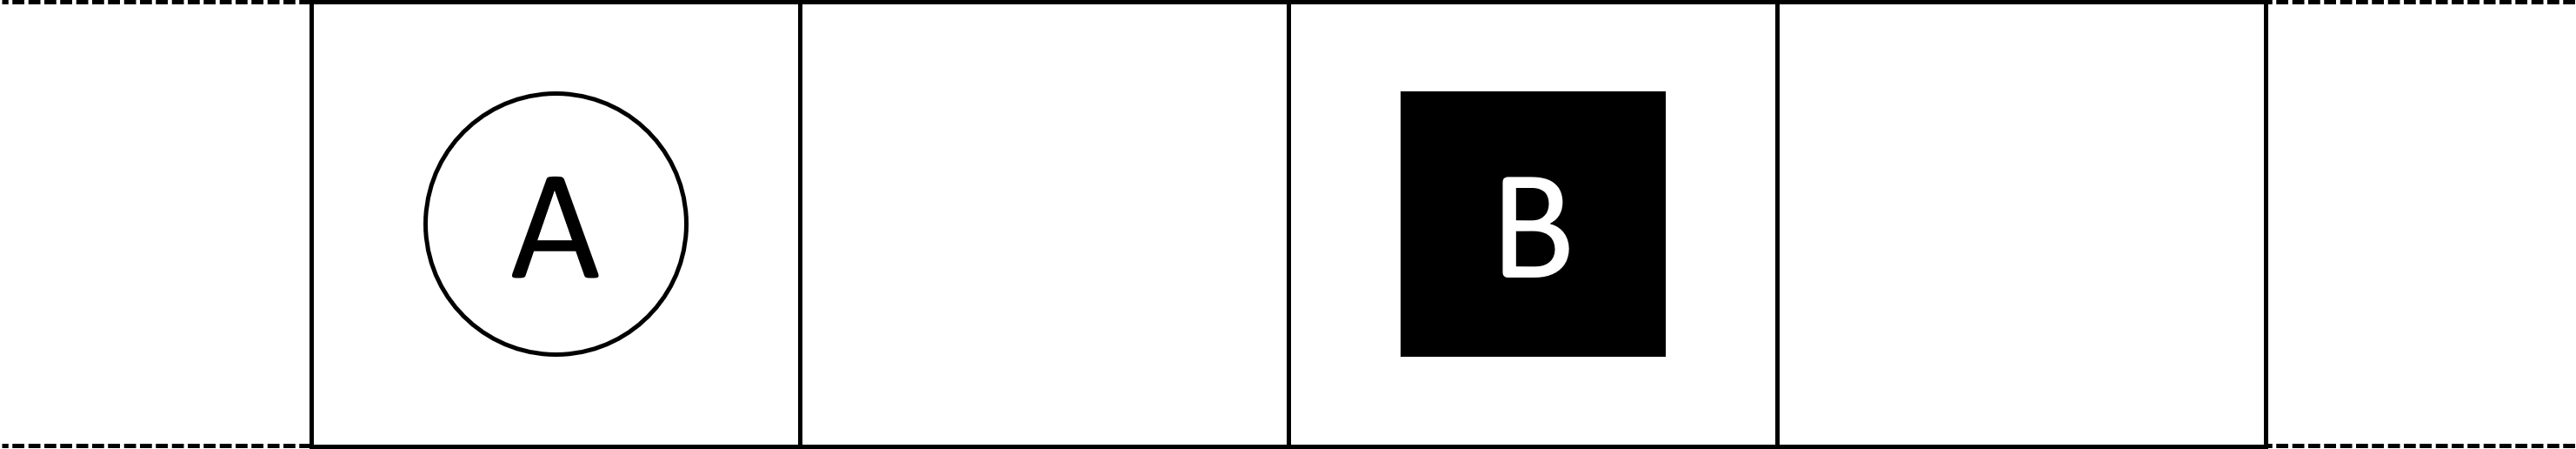
\includegraphics[width=\textwidth]{5BeyondSBDRL/Old/Images/Movable_block_world_states/w6.png}
    \caption{$w_{6}$}
  \end{subfigure}%
  \hfill
  \begin{subfigure}{0.48\textwidth}
    \centering
    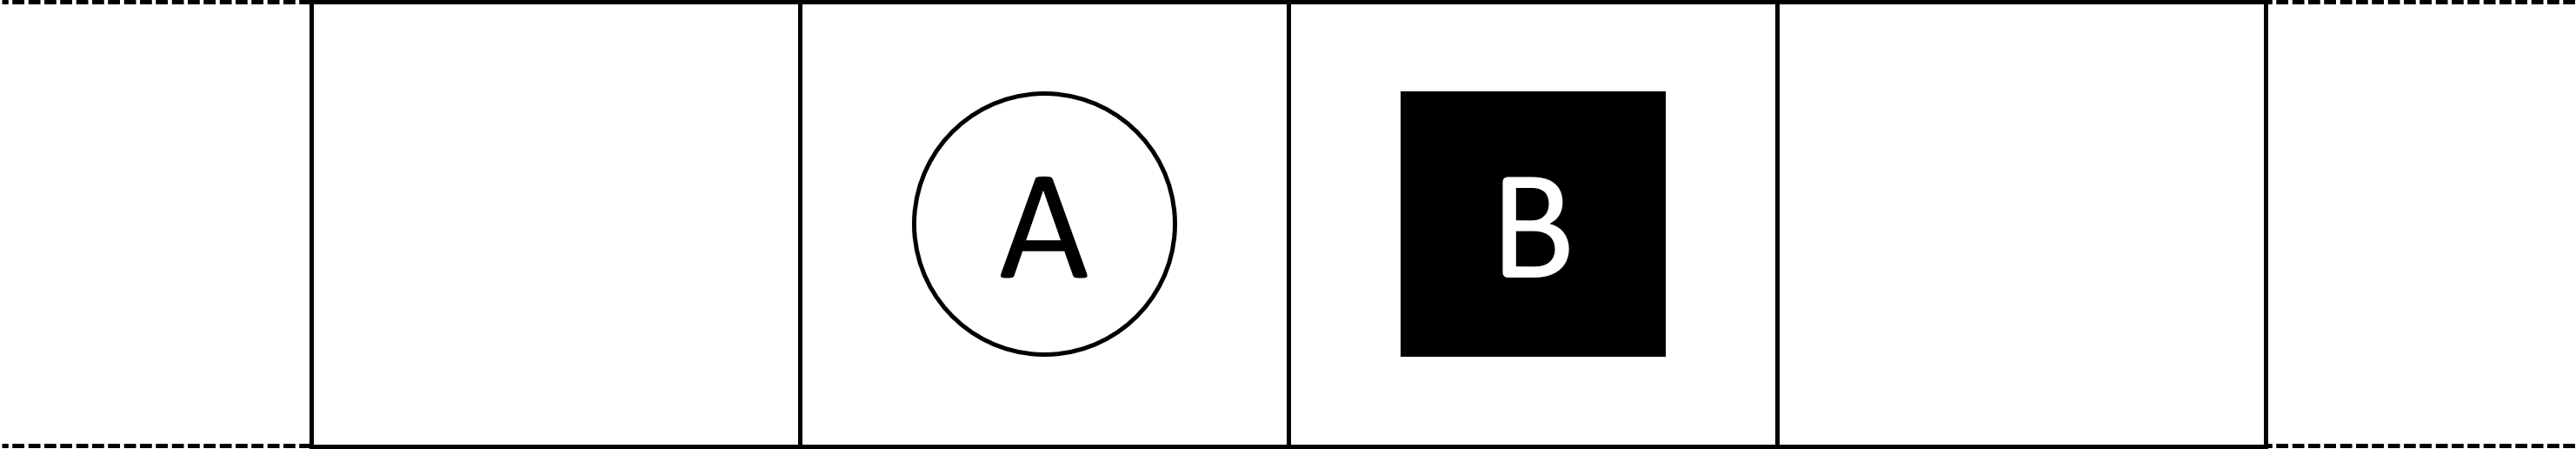
\includegraphics[width=\textwidth]{5BeyondSBDRL/Old/Images/Movable_block_world_states/w7.png}
    \caption{$w_{7}$}
  \end{subfigure}%
  \vspace{0.5cm}
  \begin{subfigure}{0.48\textwidth}
    \centering
    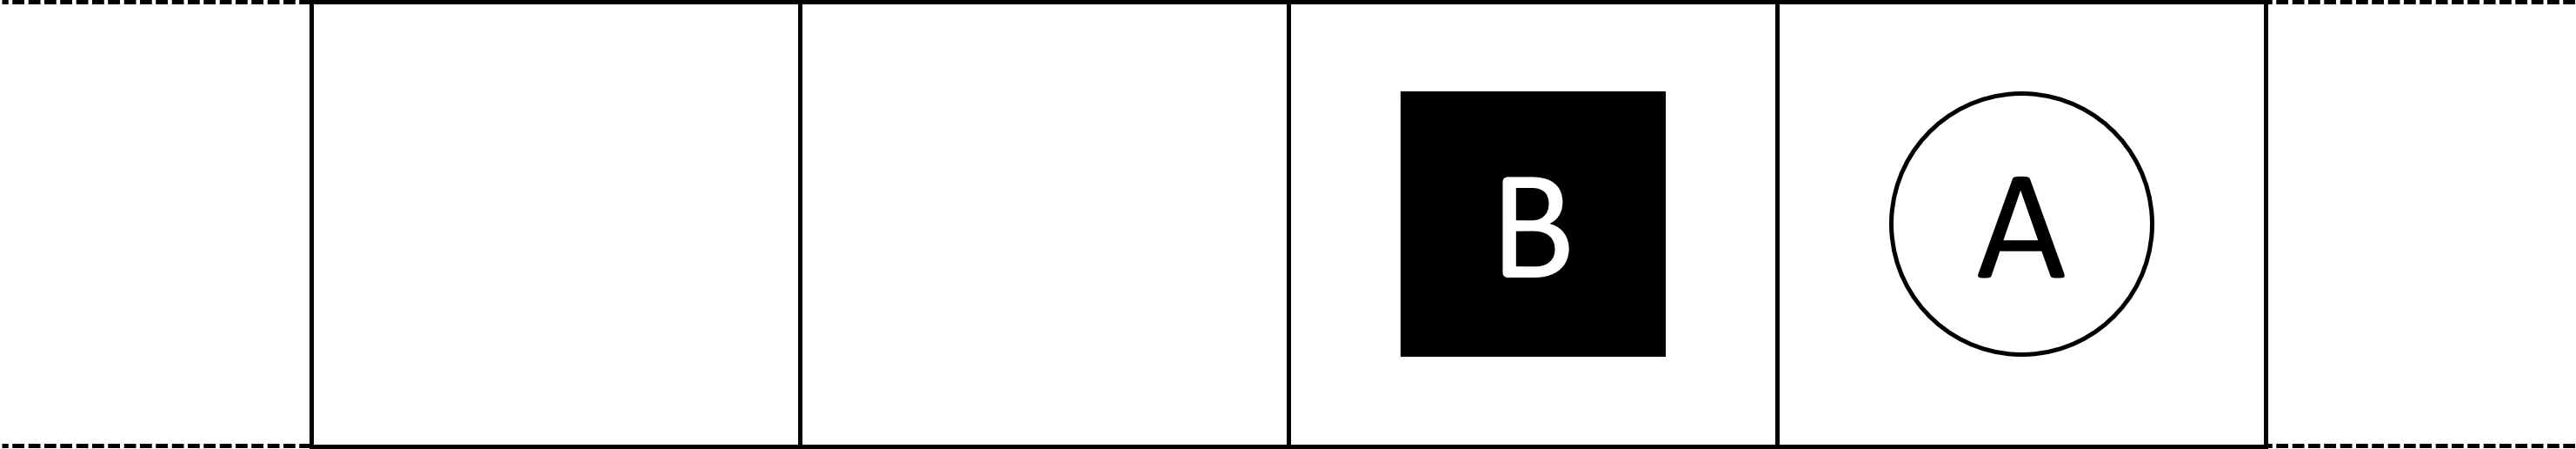
\includegraphics[width=\textwidth]{5BeyondSBDRL/Old/Images/Movable_block_world_states/w8.png}
    \caption{$w_{8}$}
  \end{subfigure}%
  \hfill
  \begin{subfigure}{0.48\textwidth}
    \centering
    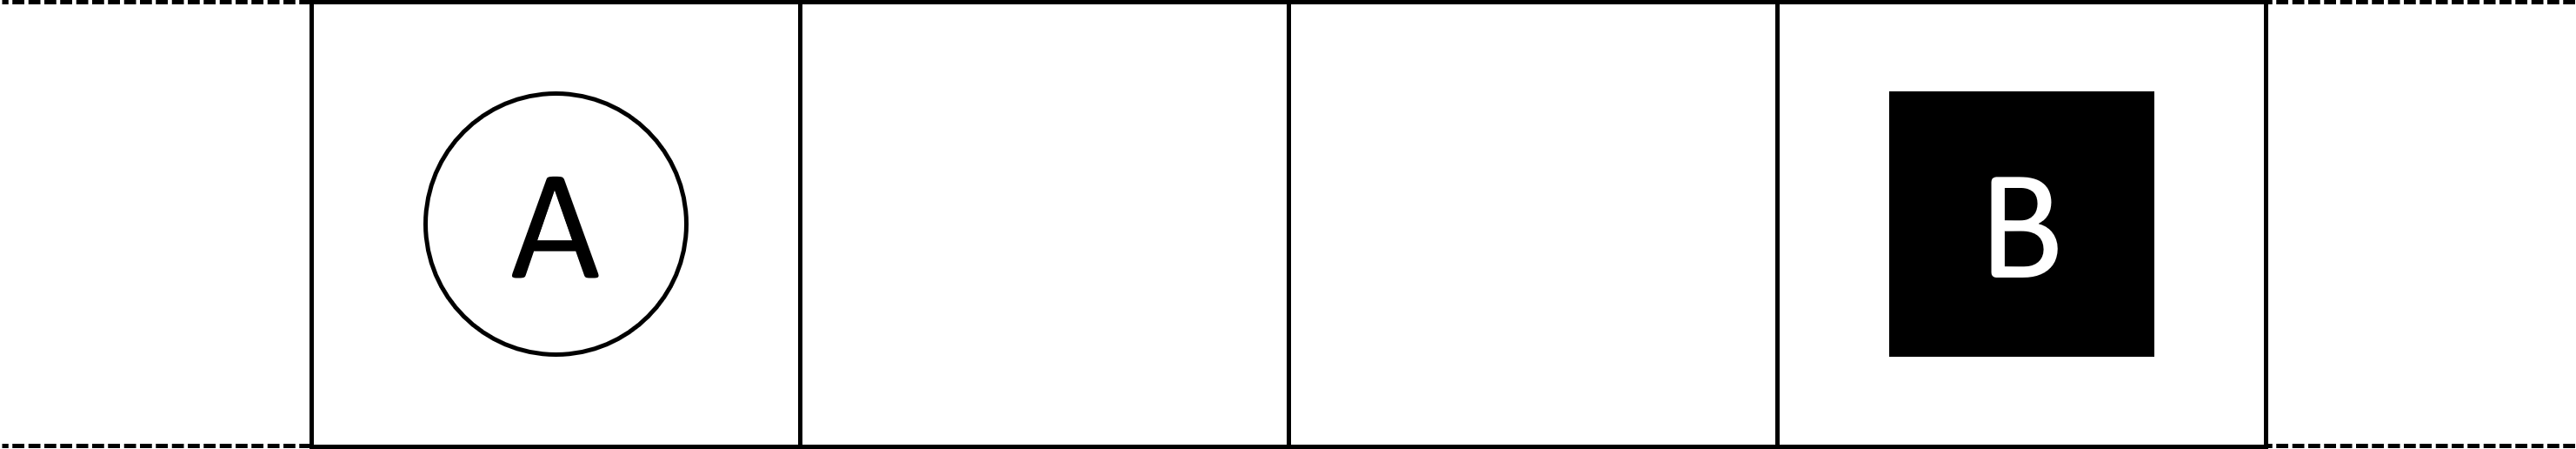
\includegraphics[width=\textwidth]{5BeyondSBDRL/Old/Images/Movable_block_world_states/w9.png}
    \caption{$w_{9}$}
  \end{subfigure}%
    \vspace{0.5cm}
  \begin{subfigure}{0.48\textwidth}
    \centering
    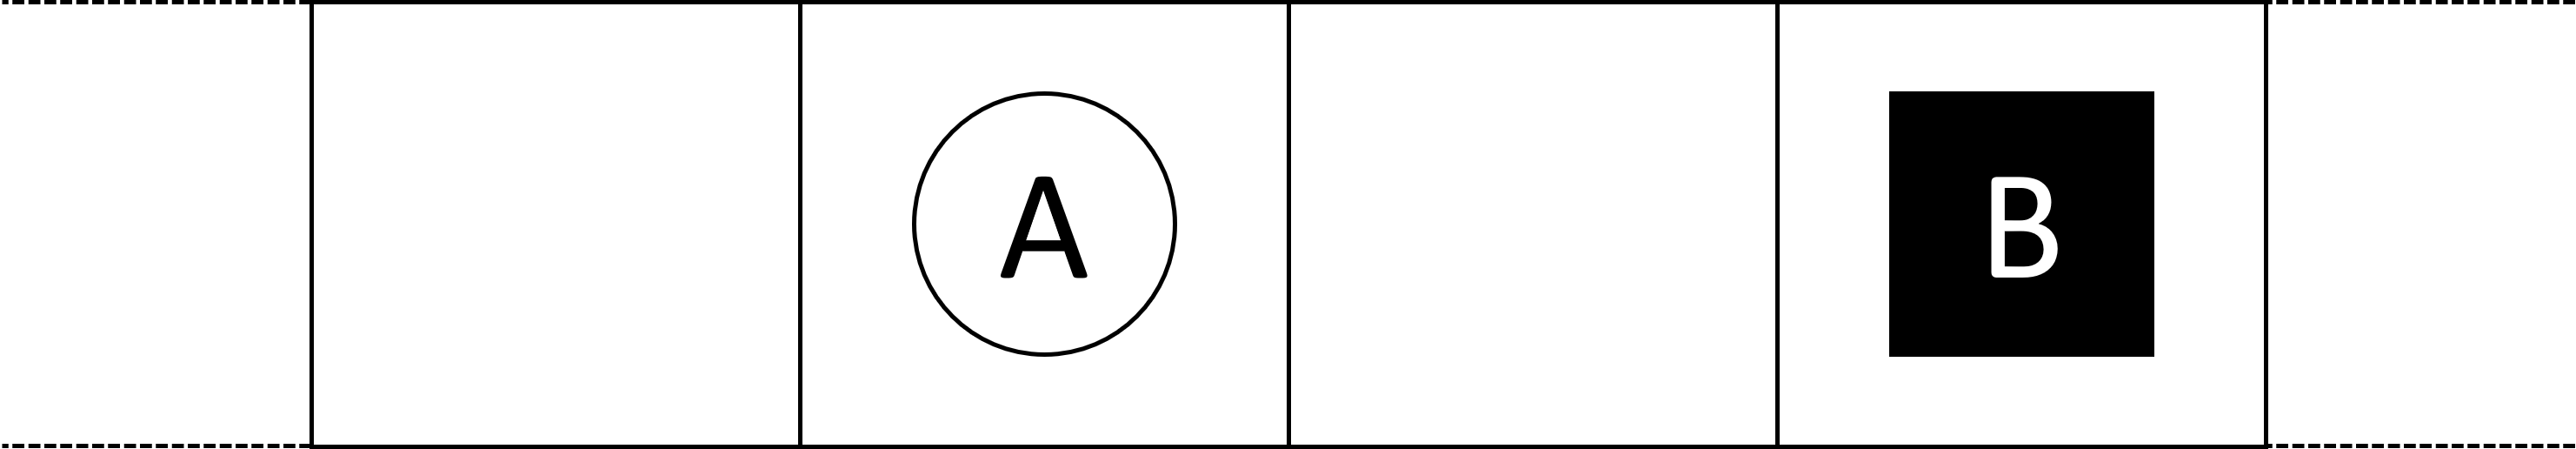
\includegraphics[width=\textwidth]{5BeyondSBDRL/Old/Images/Movable_block_world_states/w10.png}
    \caption{$w_{10}$}
  \end{subfigure}%
  \hfill
  \begin{subfigure}{0.48\textwidth}
    \centering
    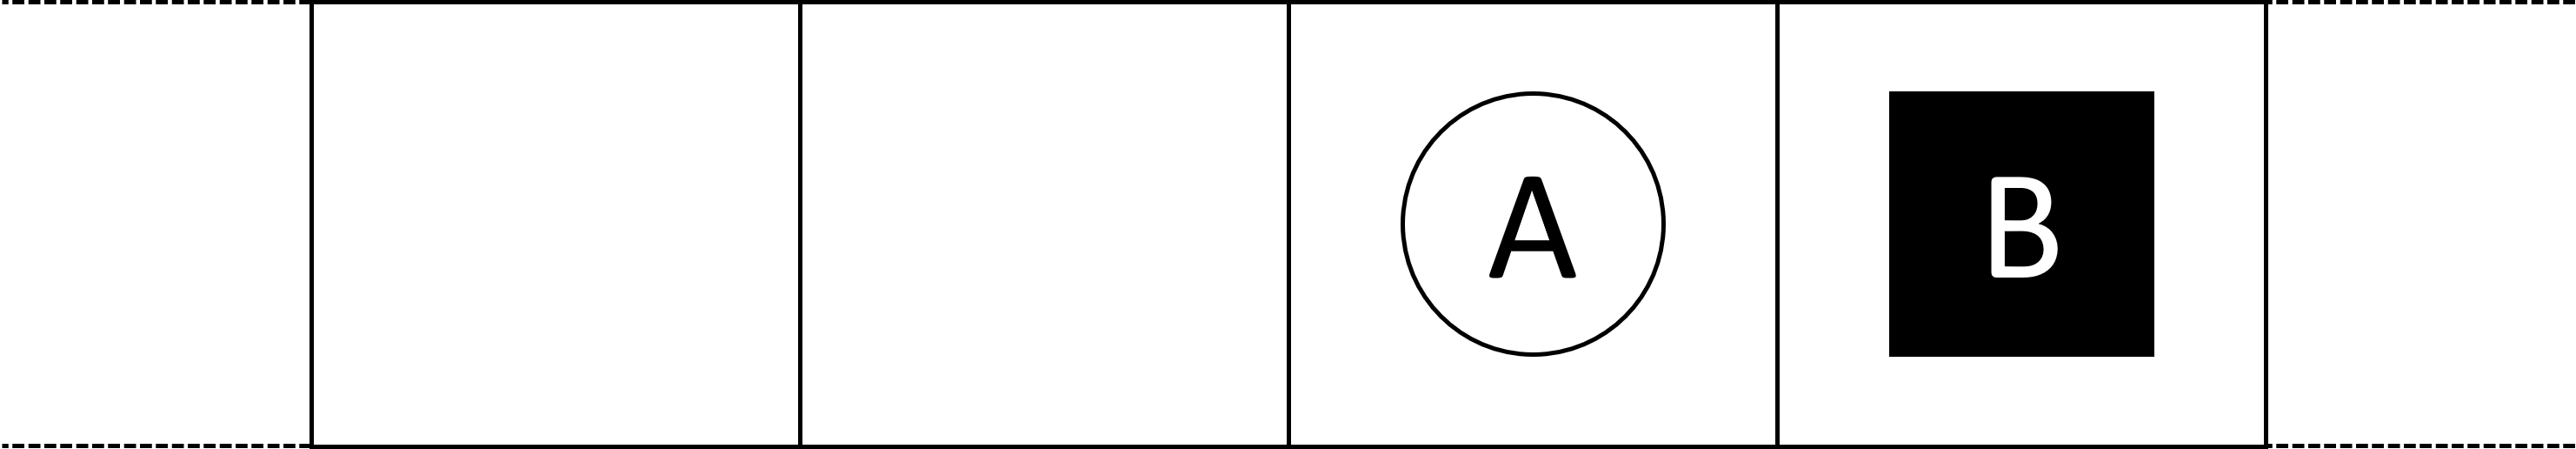
\includegraphics[width=\textwidth]{5BeyondSBDRL/Old/Images/Movable_block_world_states/w11.png}
    \caption{$w_{11}$}
  \end{subfigure}%
  \caption{World states of a world containing an agent and a movable block.}
  \label{fig:movable_block_world_states}
\end{figure}

\begin{table}[H]
    \centering
    \begin{tabular}{c|c c c c c}
                &  $1$      & $L$      & $R$\\
         \hline
        $w_{0}$ & $w_{0}$   & $w_{9}$   & $w_{1}$\\
        $w_{1}$ & $w_{1}$   & $w_{0}$   & $w_{2}$\\
        $w_{2}$ & $w_{2}$   & $w_{1}$   & $w_{3}$\\
        $w_{3}$ & $w_{3}$   & $w_{5}$   & $w_{7}$\\
        $w_{4}$ & $w_{4}$   & $w_{0}$   & $w_{5}$\\
        $w_{5}$ & $w_{5}$   & $w_{4}$   & $w_{3}$\\
        $w_{6}$ & $w_{6}$   & $w_{8}$   & $w_{7}$\\
        $w_{7}$ & $w_{7}$   & $w_{6}$   & $w_{11}$\\
        $w_{8}$ & $w_{8}$   & $w_{4}$   & $w_{6}$\\
        $w_{9}$ & $w_{9}$   & $w_{8}$   & $w_{10}$\\
        $w_{10}$ & $w_{10}$ & $w_{9}$   & $w_{11}$\\
        $w_{11}$ & $w_{11}$ & $w_{10}$  & $w_{2}$\\
    \end{tabular}
    \caption{
    Each entry in this table shows the outcome state of the agent performing the action given in the column label when in the world state given by the row label.
    }
    \label{tab:4x1-gridworld-minimum-transitions-moveable-block}
\end{table}

\begin{figure}[H]
    \centering
    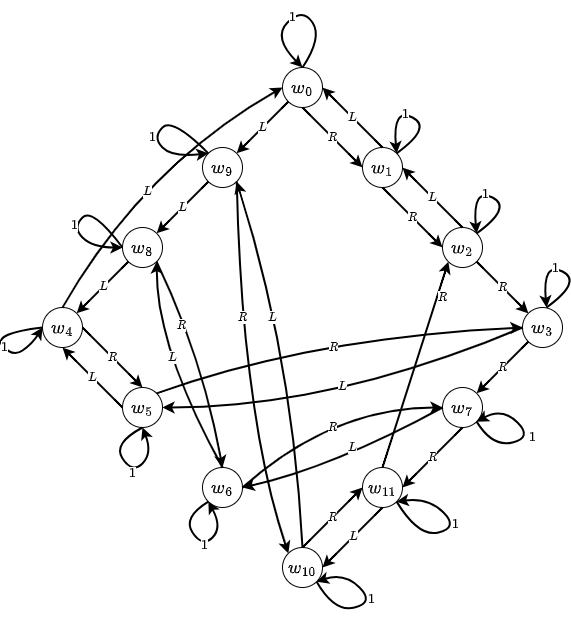
\includegraphics[width=0.7\linewidth]{5BeyondSBDRL/Old/Images/fig-4x1-block-min-actions-wall.png}
    \caption{
    A transition diagram of the labelled transitions in Table \ref{tab:4x1-gridworld-minimum-transitions-moveable-block}.
    }
    \label{fig:4x1-block-min-actions-wall}
\end{figure}

The action Cayley table for $\mathscr{W}_{block}$ contains 17 elements.
As shown by Table \ref{tab:block-world-properties}, $A/\sim$ is a monoid.

\begin{table}[H]
    \centering
    \begin{tabular}{c|c}
        \textbf{Property}   & \textbf{Present?} \\
        \hline
        Totality            & Y\\
        Identity            & Y\\
        Inverse             & N\\
        Associative         & Y\\
        Commutative         & N
    \end{tabular}
    \caption{Properties of the $A/\sim$ algebra.}
    \label{tab:block-world-properties}
\end{table}

\begin{remark}
    Adding a wall or a moveable block breaks the symmetry of the original $2 \times 2$ cyclical world $\mathscr{W}_{c}$; this manifests as the action algebra of the world being much more complex.
\end{remark}

%%%%%%%%%%%%%%%%%%%%%%%%%%%%%%%%%%%%%%%%%%%%%%%%%%%%%%%%%%%%%%
\subsection{Example 3: irreversible inhomogeneous actions}\label{sec:identity irreversible inhomogeneous actions}

This example explores the transition algebras of worlds that are action-inhomogeneous and contain irreversible actions.

Consider a world $\mathscr{W}_{consumable}$ with movement along a single 1D cyclical axis with a single consumable.
Let this world also contain an agent that can move left, right or consume the consumable if the agent is in the same place as the consumable.

\begin{figure}[H]
  \centering
  \begin{subfigure}{0.48\textwidth}
    \centering
    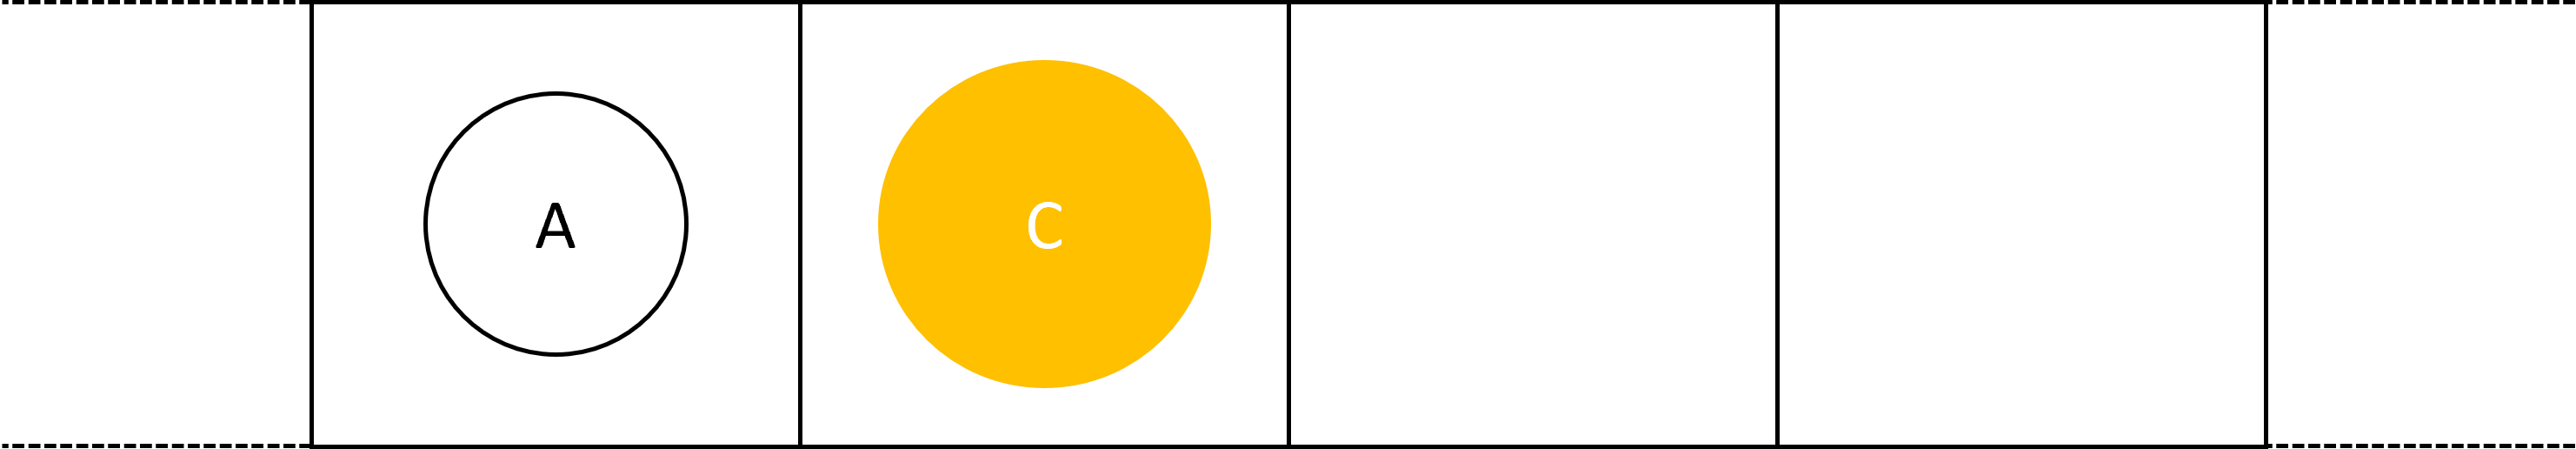
\includegraphics[width=\textwidth]{5BeyondSBDRL/Old/Images/Consumable_world_states/w0.png}
    \caption{$w_{0}$}
    \label{fig:w0}
  \end{subfigure}%
  \hfill
  \begin{subfigure}{0.48\textwidth}
    \centering
    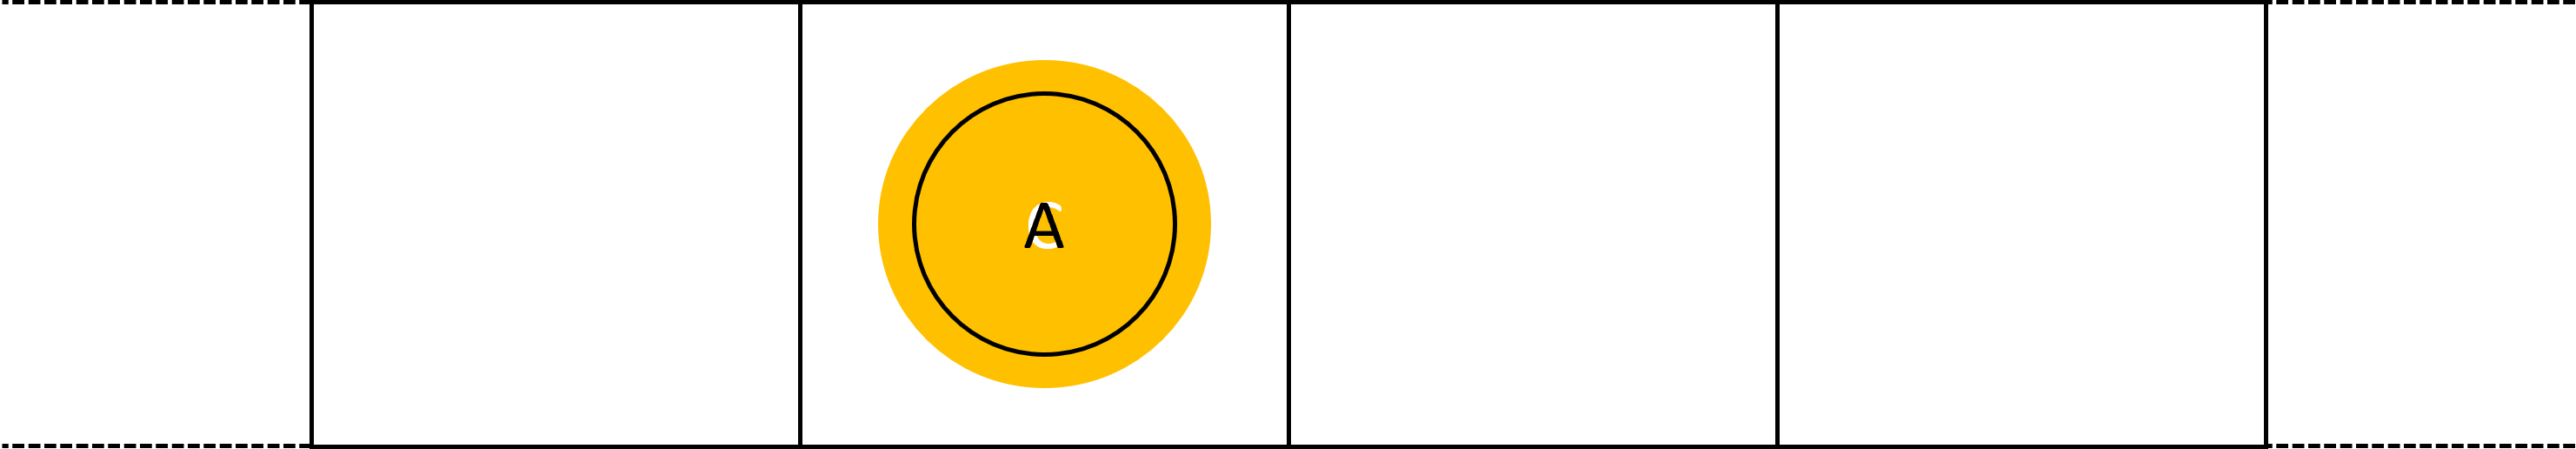
\includegraphics[width=\textwidth]{5BeyondSBDRL/Old/Images/Consumable_world_states/w1.png}
    \caption{$w_{1}$}
    \label{fig:w1}
  \end{subfigure}%
  \vspace{0.5cm}
  \begin{subfigure}{0.48\textwidth}
    \centering
    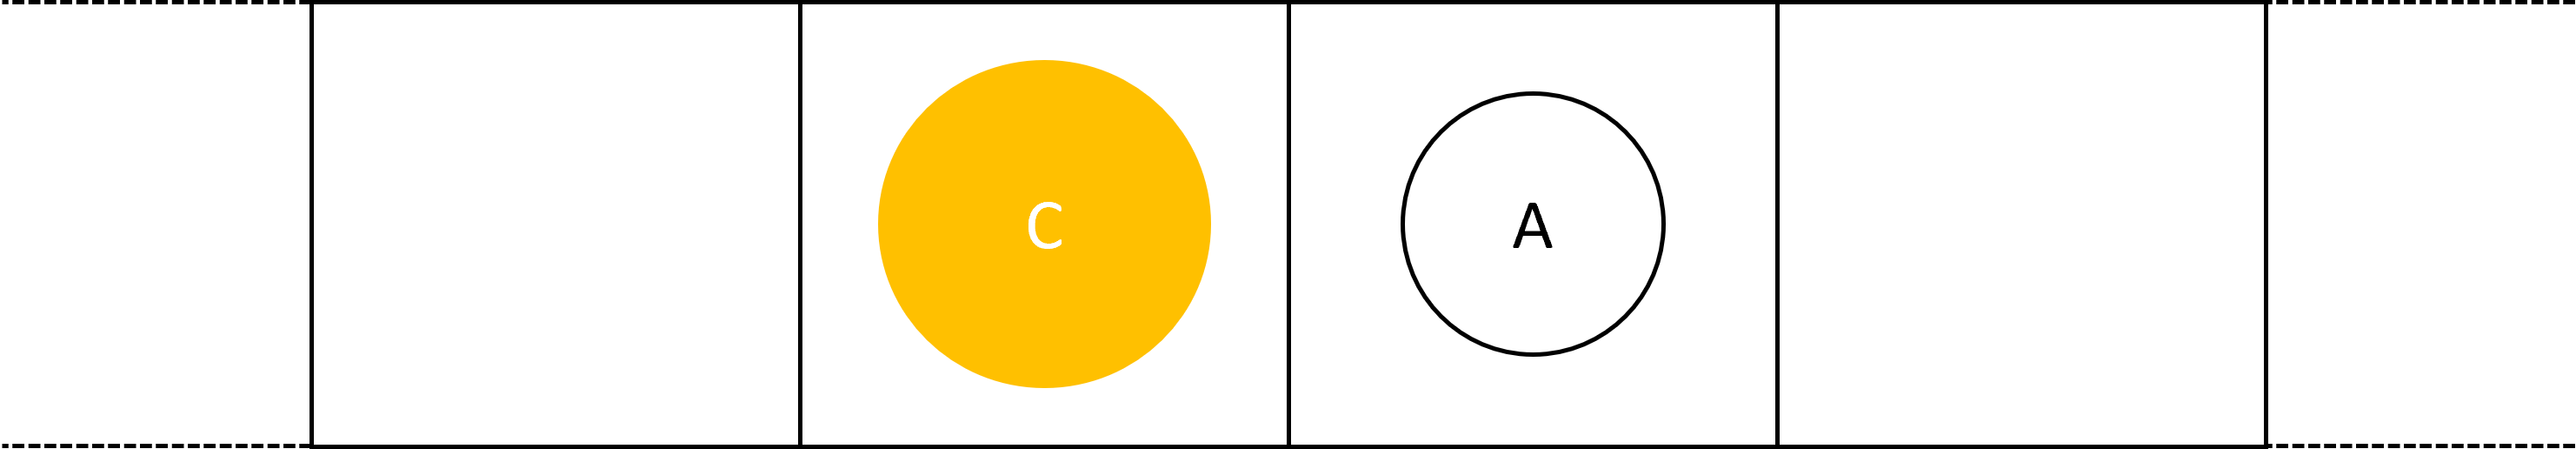
\includegraphics[width=\textwidth]{5BeyondSBDRL/Old/Images/Consumable_world_states/w2.png}
    \caption{$w_{2}$}
    \label{fig:w2}
  \end{subfigure}%
  \hfill
  \begin{subfigure}{0.48\textwidth}
    \centering
    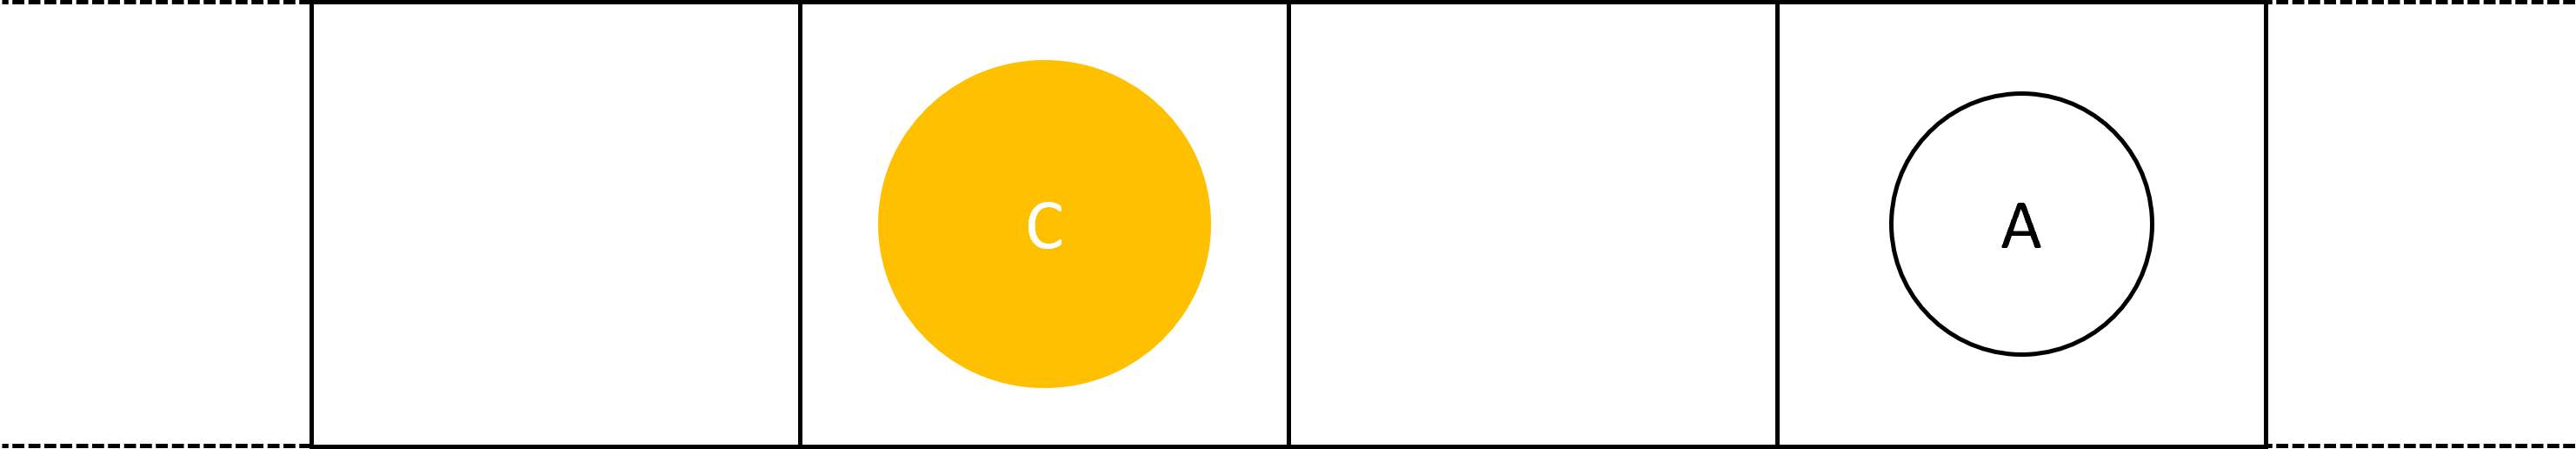
\includegraphics[width=\textwidth]{5BeyondSBDRL/Old/Images/Consumable_world_states/w3.png}
    \caption{$w_{3}$}
    \label{fig:w3}
  \end{subfigure}%
  \vspace{0.5cm}
  \begin{subfigure}{0.48\textwidth}
    \centering
    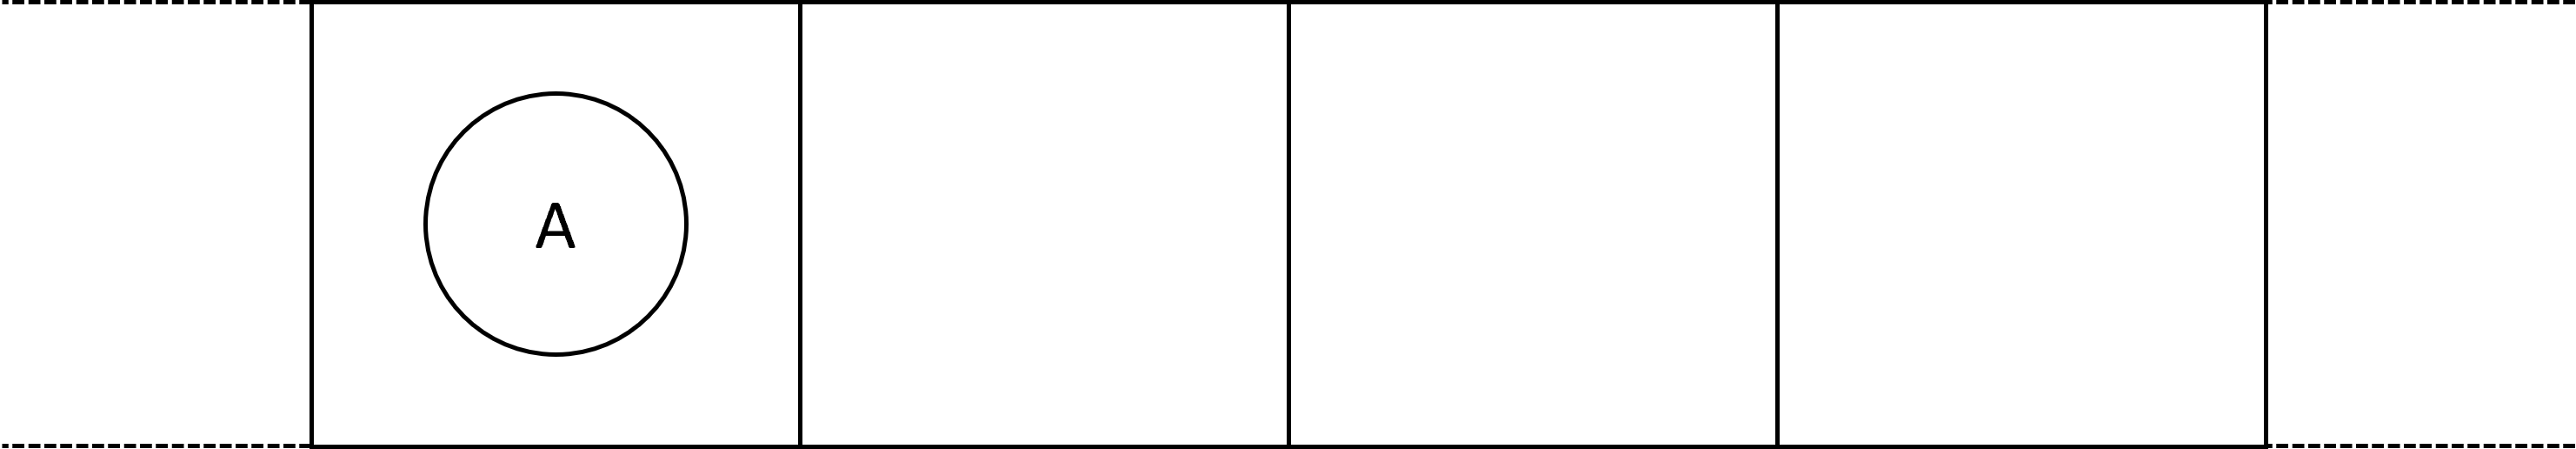
\includegraphics[width=\textwidth]{5BeyondSBDRL/Old/Images/Consumable_world_states/w4.png}
    \caption{$w_{4}$}
    \label{fig:w4}
  \end{subfigure}%
  \hfill
  \begin{subfigure}{0.48\textwidth}
    \centering
    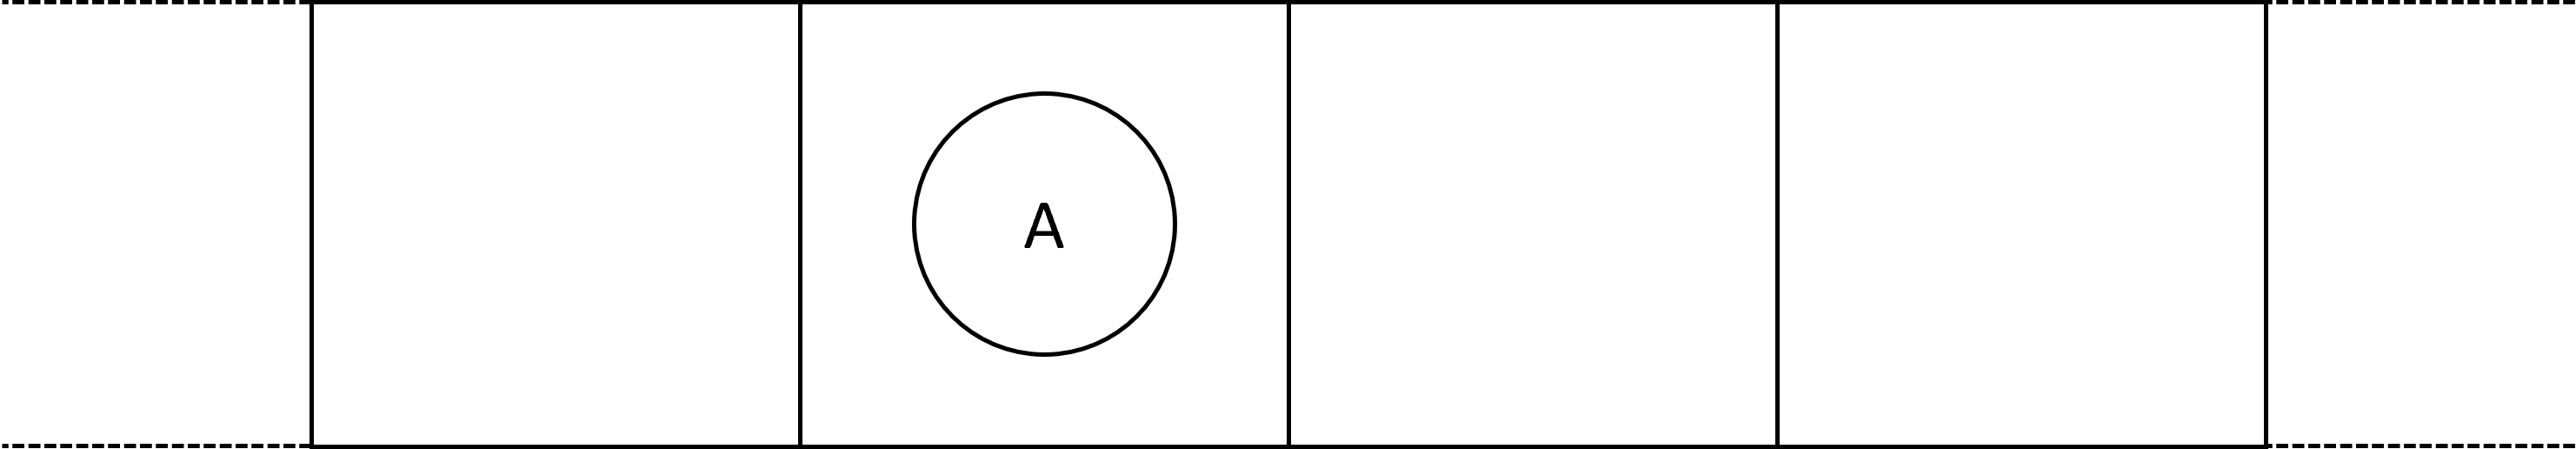
\includegraphics[width=\textwidth]{5BeyondSBDRL/Old/Images/Consumable_world_states/w5.png}
    \caption{$w_{5}$}
    \label{fig:w5}
  \end{subfigure}%
  \vspace{0.5cm}
  \begin{subfigure}{0.48\textwidth}
    \centering
    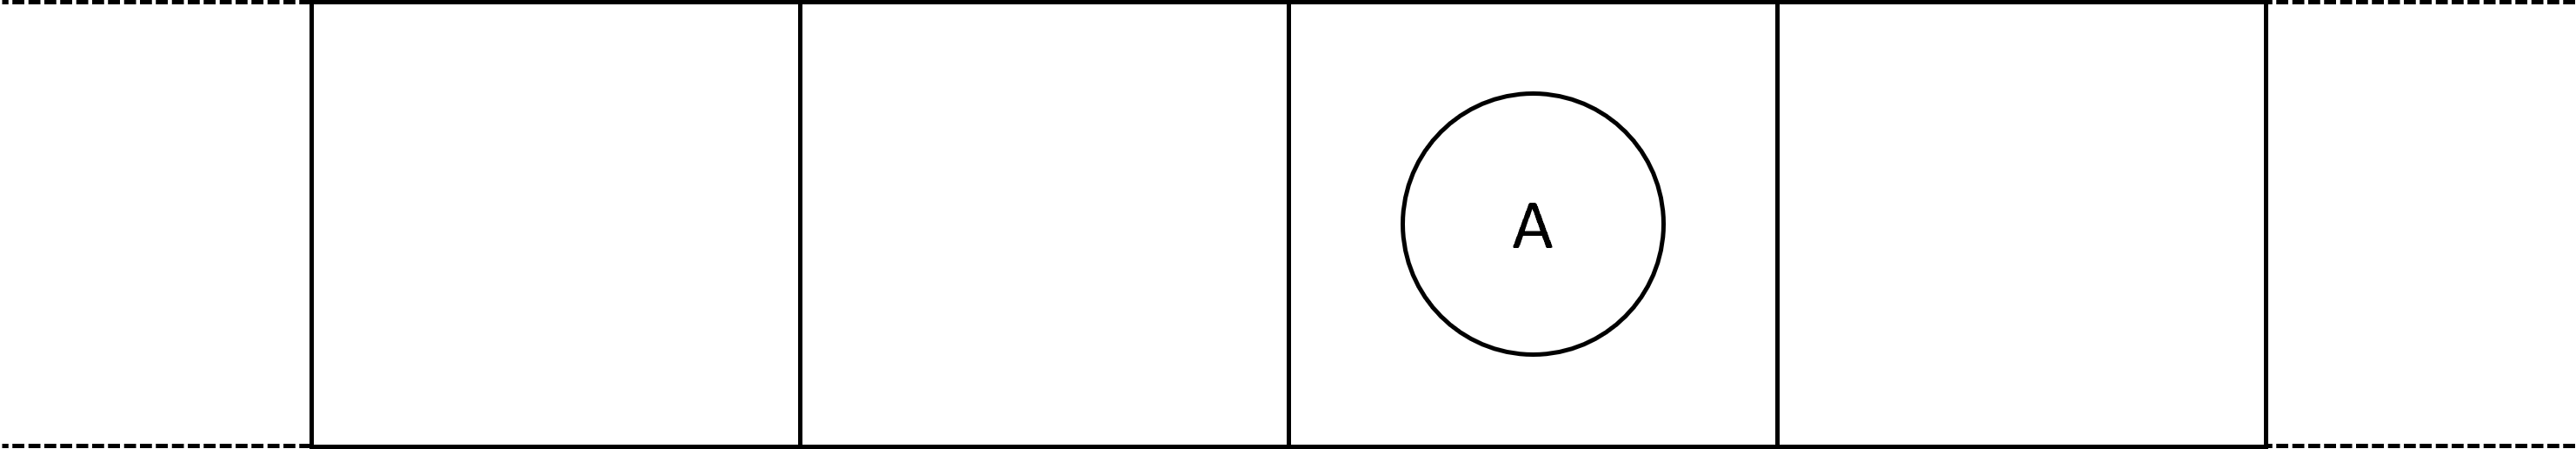
\includegraphics[width=\textwidth]{5BeyondSBDRL/Old/Images/Consumable_world_states/w6.png}
    \caption{$w_{6}$}
    \label{fig:w6}
  \end{subfigure}%
  \hfill
  \begin{subfigure}{0.48\textwidth}
    \centering
    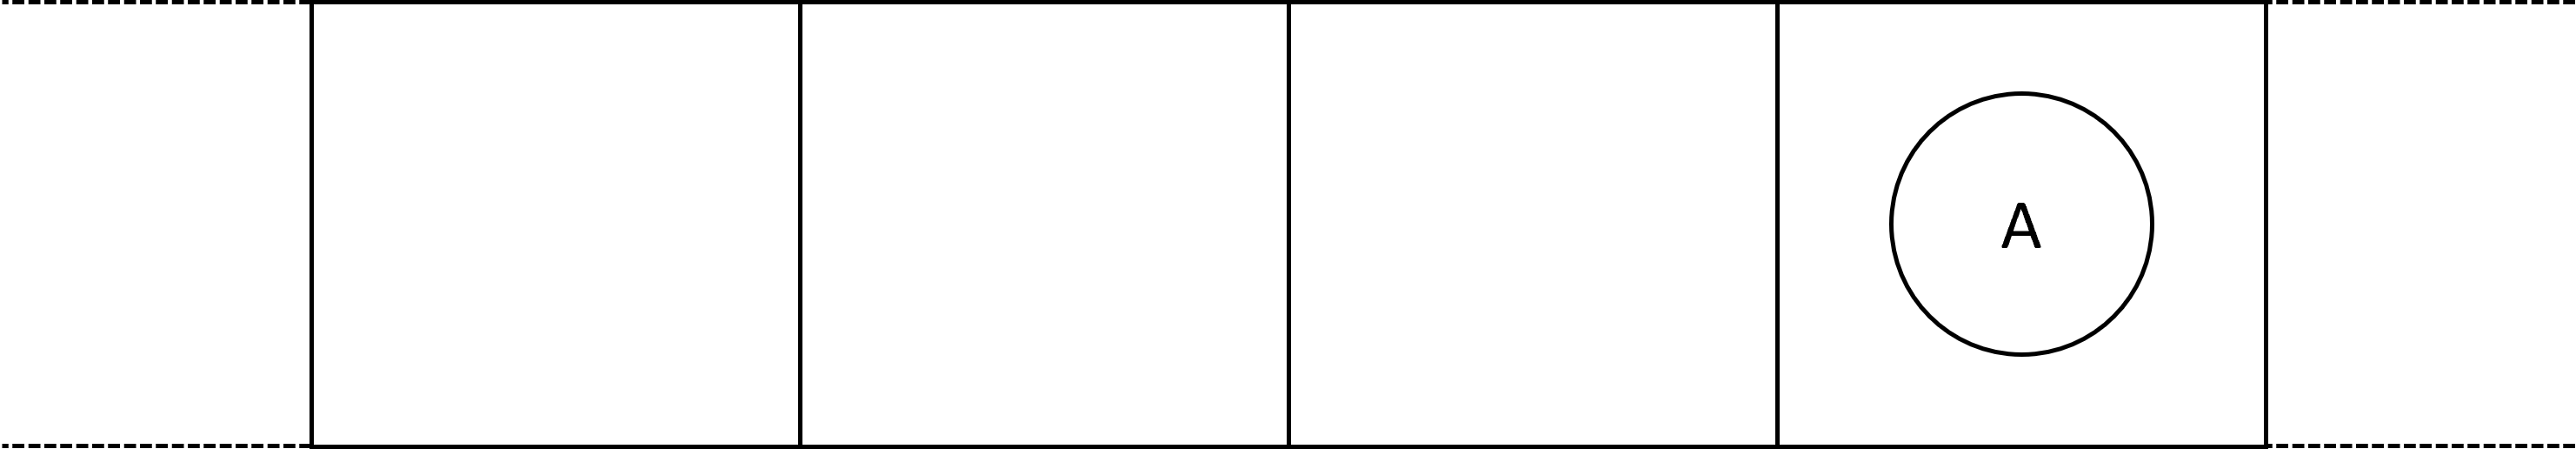
\includegraphics[width=\textwidth]{5BeyondSBDRL/Old/Images/Consumable_world_states/w7.png}
    \caption{$w_{7}$}
    \label{fig:w7}
  \end{subfigure}%
  
  \caption{World states of a world containing an agent and a consumable.}
  \label{fig:consumable_world_states}
\end{figure}

There is not a consumable in every state, therefore if the agent performs the consume action in any state except $w_{1}$ then the effect will be the same as if the agent had performed the no-op action $1 \in A/\sim$ (see Figure \ref{fig:min-action-net-world-with-consumable-identity}).

\begin{figure}[H]
    \centering
    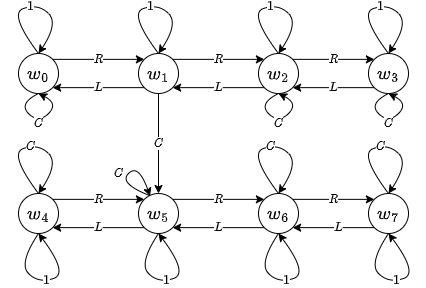
\includegraphics[width=0.7\linewidth]{5BeyondSBDRL/Old/Images/fig-min-action-net-world-with-consumable-identity.png}
    \caption{
   Minimum action network for world $\mathscr{W}_{consumable}$.
    }
    \label{fig:min-action-net-world-with-consumable-identity}
\end{figure}

The action Cayley table for world $\mathscr{W}_{consumable}$ with restricted actions treated as identity actions contains 64 elements.
As shown in Table \ref{tab:identity-consumable-properties}, $A/\sim$ is a monoid.

\begin{table}[H]
    \centering
    \begin{tabular}{c|c}
        \textbf{Property}   & \textbf{Present?} \\
        \hline
        Totality            & Y\\
        Identity            & Y\\
        Inverse             & N\\
        Associative         & Y\\
        Commutative         & N
    \end{tabular}
    \caption{Properties of the $A/\sim$ algebra.}
    \label{tab:identity-consumable-properties}
\end{table}

\begin{remark}
    Considering this example, we note that the irreversible action moves from one `reversible plane' to another.
    Perhaps we can treat an irreversible action as having a `reversible action affecting part' and a `world affecting part'; in this example, the reversible action affecting part would be the identity action since the reversible action network is unchanged by the irreversible action.
\end{remark}

%%%%%%%%%%%%%%%%%%%%%%%%%%%%%%%%%%%%%%%%%%%%%%%%%%%%%%%%%%%%%%%%%%%%%%%%%%%%%%
\subsection{Worlds without inverse actions or unrestricted actions}\label{sec:Worlds without inverse actions or unrestricted actions}

In this section, we consider worlds that do not necessarily satisfy world condition ref[wldcon:inverse-actions] or world condition ref[wldcon:unrestricted-actions].

\begin{proposition}\label{prp:all_worlds_give_small_category_action}
    Consider a world $\mathscr{W}$ with a set $W$ of world states and containing an agent with a set $A$ of actions.
    $*: (A/\sim) \times W \to W'$, where $W' \subseteq W$, is the action of a small category $A/\sim$ on $W$.
\end{proposition}
\begin{proof}
    (1) Associativity of $A/\sim$ is given by proposition ref[prp:Asim-associative].
    (2) Identity element of $A/\sim$ is given by proposition ref[prp:Asim-identity].
    Since $A/\sim$ satisfies properties (1) and (2), $A/\sim$ is a small category.
    Therefore $*$ is the action of a small category.
\end{proof}

\begin{remark}
    We can consider two equivalent perspectives of $*$:
    \begin{enumerate}
        \item $A/\sim$ is a small category and $*$ is a full action of $A/\sim$ on $W$.
        \item $A/\sim$ is a monoid and $*$ is a partial action of $A/\sim$ on $W$.
    \end{enumerate}
\end{remark}

%%%%%%%%%%%%%%%%%%%%%%%%%%%%%%%%%%%%%%
\subsection{Example 1: reversible action-inhomogeneous world}\label{sec:masked reversible action-inhomogeneous world}

We once again consider the world $\mathscr{W}_{wall}$ (see Figure \ref{fig:2x2-cyclical-grid-world-wall-states} for world states); however, now instead of treating restricted actions like the identity action, we \textit{mask} the restricted actions.
Masking restricted actions involves not allowing the agent to perform the restricted actions - the restricted actions are hidden (masked) from the agent - and so, mathematically, we treat the restricted actions as \textit{undefined}; for example, if $\mathscr{W}_{wall}$ is in state $w_{0}$, then the agent cannot perform the $R$ action because $R * w_{0}$ is undefined.

\begin{table}[H]
    \centering
    \begin{tabular}{c|c c c c c}
                &  $1$      & $U$       & $D$       & $L$               & $R$\\
         \hline
        $w_{0}$ & $w_{0}$   & $w_{2}$   & $w_{2}$   & $w_{1}$           & undefined\\
        $w_{1}$ & $w_{1}$   & $w_{3}$   & $w_{3}$   & undefined         & $w_{0}$\\
        $w_{2}$ & $w_{2}$   & $w_{0}$   & $w_{0}$   & $w_{3}$           & $w_{3}$\\
        $w_{3}$ & $w_{3}$   & $w_{1}$   & $w_{1}$   & $w_{2}$           & $w_{2}$\\
    \end{tabular}
    \caption{Each entry in this table shows the outcome state of the agent performing the action given in the column label when in the world state given by the row label.}
    \label{tab:2x2-gridworld-minimum-transition-wall-masked}
\end{table}

\begin{figure}[H]
    \centering
    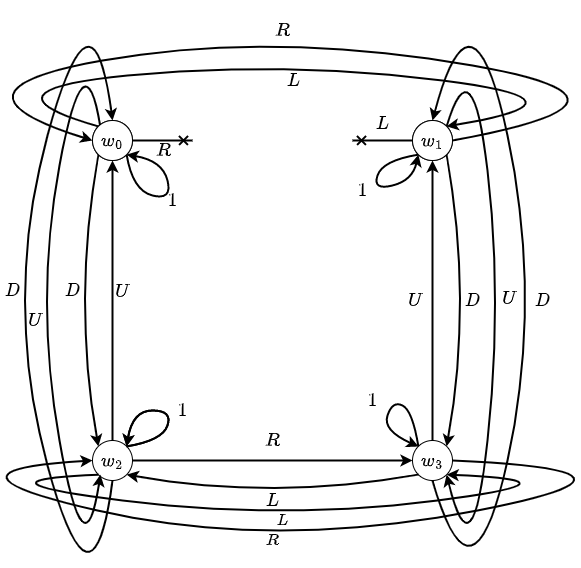
\includegraphics[width=0.5\linewidth]{5BeyondSBDRL/Old/Images/restricted-walls-2x2-cyclical-min-actions.drawio.png}
    \caption{
    A diagram of the labelled transitions in Table \ref{tab:2x2-gridworld-minimum-transition-wall-masked}.
    }
    \label{fig:2x2-cyclical-min-actions-wall-masked}
\end{figure}

The action Cayley table for $\mathscr{W}_{wall}$ with the masked treatment of the walls contains 59 elements.
As shown in Table \ref{tab:masked-walls}, $A/\sim$ is a small category.

\begin{table}[H]
    \centering
    \begin{tabular}{c|c}
        \textbf{Property}   & \textbf{Present?} \\
        \hline
        Totality            & N\\
        Identity            & Y\\
        Inverse             & N\\
        Associative         & Y\\
        Commutative         & N
    \end{tabular}
    \caption{Properties of the $A/\sim$ algebra.}
    \label{tab:masked-walls}
\end{table}

%%%%%%%%%%%%%%%%%%%%%%%%%%%%%%%%%%%%%%
\subsection{Example 2: irreversible action-inhomogeneous world}\label{sec:masked irreversible action-inhomogeneous world}

We will now apply the masking treatment of restricted actions to the world $\mathscr{W}_{consumable}$ (see Figure \ref{fig:consumable_world_states} for world states); for example, if $\mathscr{W}_{consumable}$ is not in state $w_{1}$ then the consume action is undefined.

\begin{figure}[H]
    \centering
    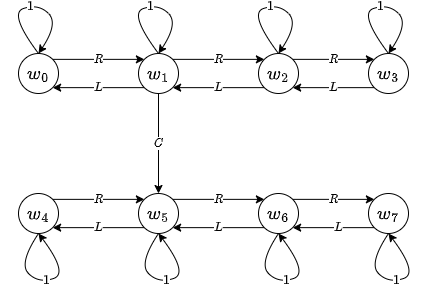
\includegraphics[scale=0.5]{5BeyondSBDRL/Old/Images/fig-min-action-net-world-with-consumable-masked.png}
    \caption{Minimum action network for world containing an agent and a consumable.}
    \label{fig-min-action-net-world-with-consumable-masked}
\end{figure}

The action Cayley table for $\mathscr{W}_{consumable}$ with the masked treatment of the walls contains 20 elements.
As shown in Table \ref{tab:masked-consumable-properties}, $A/\sim$ is a small category.

\begin{table}[H]
    \centering
    \begin{tabular}{c|c}
        \textbf{Property}   & \textbf{Present?} \\
        \hline
        Totality            & N\\
        Identity            & Y\\
        Inverse             & N\\
        Associative         & Y\\
        Commutative         & N
    \end{tabular}
    \caption{Properties of the $A/\sim$ algebra.}
    \label{tab:masked-consumable-properties}
\end{table}

\begin{remark}
    For any world, once the agent has the action Cayley table for any initial world state it can produce the action Cayley table for any other initial world state by applying an action that transitions from the old initial world state to the new initial world state to every element of the action Cayley table.
\end{remark}

\begin{proposition}\label{prp:algebra_depends_on_action_treatment}
    The algebra $A/\sim$ of the actions of an agent depends on the treatment of the actions of the agent (\textit{e.g.}, masked treatment vs identity treatment) even if the world states remain the same.
\end{proposition}
\begin{proof}
    $A/\sim$ for the identity treatment of $\mathscr{W}_{wall}$ contains 26 elements, while $A/\sim$ for the masked treatment of $\mathscr{W}_{wall}$ contains 59 elements.

    Additionally, $A/\sim$ for the identity treatment of $\mathscr{W}_{consumable}$ contains 64 elements, while $A/\sim$ for the masked treatment of $\mathscr{W}_{consumable}$ contains 20 elements.
\end{proof}

We have also demonstrated that neither the identity treatment nor the masked treatment produces the more simple algebra in every world.
For $\mathscr{W}_{wall}$, the identity treatment contains fewer elements than the masked treatment (26 elements vs 59 elements), while for $\mathscr{W}_{consumable}$ the masked treatment contains fewer elements than the identity treatment (20 elements vs 64 elements).


